\section{Esperimenti}
\fancyhead[RO,LE]{Esperimenti}

I grafici sottostanti sono stati generati con uno script \textit{Python} a partire da dei \texttt{.csv} esportati dall'interfaccia web, tutte queste risorse sono disponibili nella cartella \texttt{experiments} sulla \anchor{repository \textit{Github}}{https://github.com/albbus-stack/platooning-visualization/tree/main/experiments} divise in cartelle relative al parametro testato.

\begin{pyCode}{Generazione dei grafici con \textit{Matplotlib}}
def plot_and_save(output_filename, data, ylabel):
  for car_index, car_data in data.items():
    if ylabel == 'distance' and car_index == len(data.items()) - 1:
      continue
    plt.plot(car_data['time'], car_data[ylabel], marker='o', linestyle='-', 
      label=f'Auto {car_index + 1}' if ylabel == 'velocity'
        else f'Distanza {car_index + 1}-{car_index + 2}')

  plt.xlabel('Tempo (s)')
  plt.ylabel('Velocità (m/s)' if ylabel == 'velocity' else 'Distanza (m)')
  plt.legend()
  plt.savefig(output_filename)
  plt.close()
\end{pyCode}

\newpage
\subsection{Modello stabile}

% DEFAULT %

\subsubsection{Parametri di default}
Questi parametri sono presi dall'articolo \cite{ploeg_2014_lp}.

%\begin{table}[h]
%    \centering
%    \begin{tabular}{|c|c|c|c|c|}
%        \hline
%        Velocità $t1$ & Velocità $t2$ & Velocità $t3$ &Velocità $t4$ &Velocità $t5$\\
%        \hline
%            $2\hspace{0.2em}m/s$ & $4\hspace{0.2em}m/s$ & $6\hspace{0.2em}m/s$ & $8\hspace{0.2em}m/s$ & $10\hspace{0.2em}m/s$ \\
%        \hline
%    \end{tabular}
%    \label{tab:experiment_velocities}
%\end{table}
\begin{table}[h]
    \centering
    \begin{tabular}{|c|c|c|c|}
        \hline
        N° auto & Distanza Iniziale & Distanza Target & Ritardo \\
        \hline
        $6$ & $6.0 m$ & $5.0 m$ & $0.2 s$ \\
        \hline
        $Time\hspace{0.2em}Headway$ & $\tau$ & $K_p$ & $K_d$  \\
        \hline
        $0.5$ & $0.1$ & $0.2$ & $0.7$ \\
        \hline
    \end{tabular}
    \label{tab:default_parameters}
\end{table}

\begin{figure}[H]
    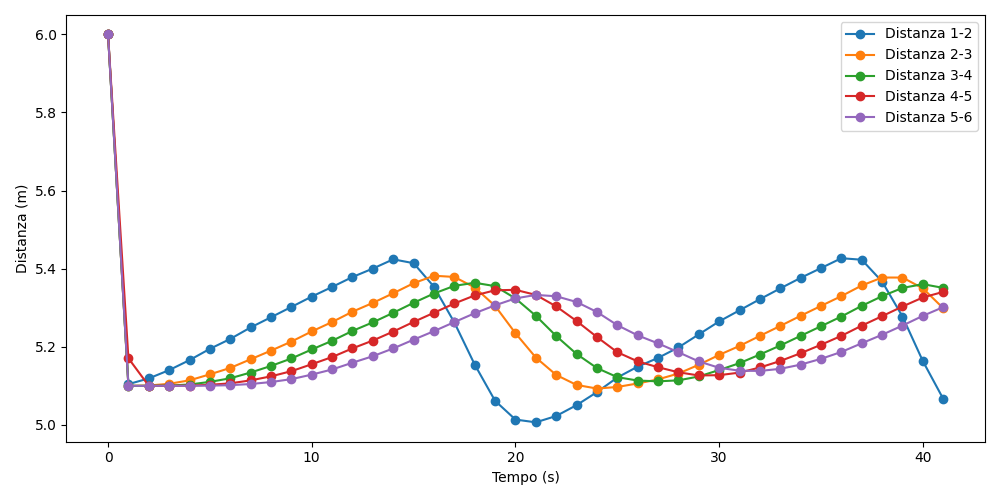
\includegraphics[width=0.96\textwidth]{images/5-experiment/default/distance_6.png}
    \caption{Distanze con parametri di default.}
    \label{fig:default-distance}
\end{figure}

\begin{figure}[H]
    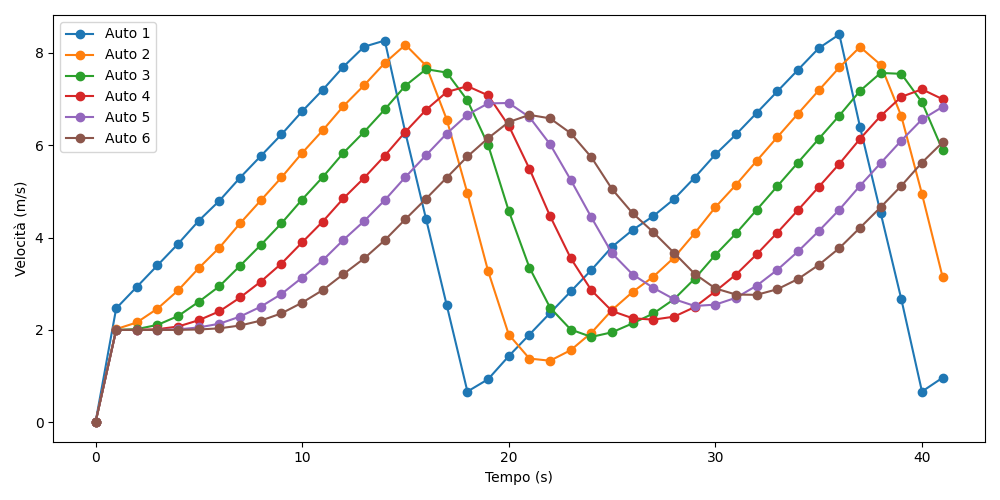
\includegraphics[width=0.96\textwidth]{images/5-experiment/default/velocity_6.png}
    \caption{Velocità con parametri di default.}
    \label{fig:default-velocity}
\end{figure}
\newpage

% CAR NUMBER %

\subsubsection{Numero di auto}
\vspace*{\fill}
\begin{table}[h]
    \centering
    \begin{tabular}{|c|c|c|c|}
        \hline
        N° auto & Distanza Iniziale & Distanza Target & Ritardo \\
        \hline
        $3$ & $6.0 m$ & $5.0 m$ & $0.2 s$ \\
        \hline
        $Time\hspace{0.2em}Headway$ & $\tau$ & $K_p$ & $K_d$  \\
        \hline
        $0.5$ & $0.1$ & $0.2$ & $0.7$ \\
        \hline
    \end{tabular}
\end{table}

\begin{figure}[H]
    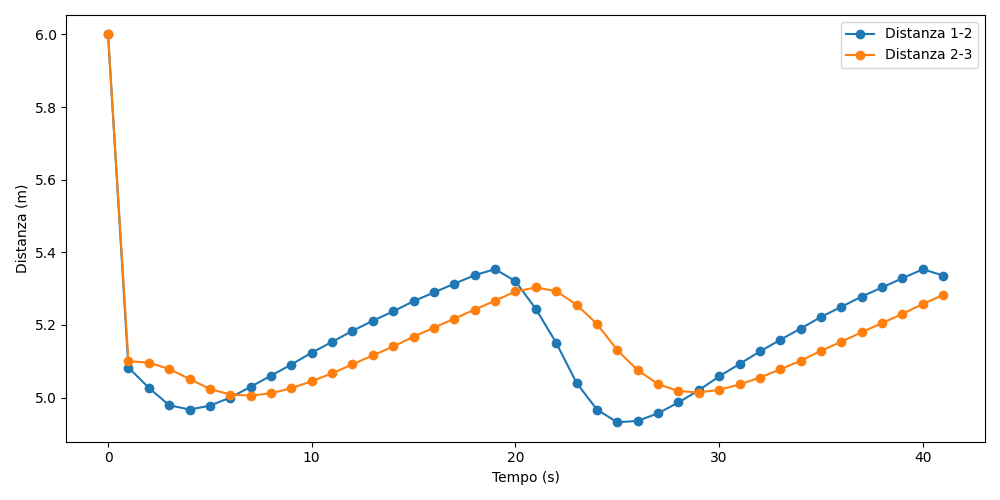
\includegraphics[width=0.96\textwidth]{images/5-experiment/car-number/distance_3.png}
    \caption{Distanze con 3 auto.}
    \label{fig:3-cars-distance}
\end{figure}

\begin{figure}[H]
    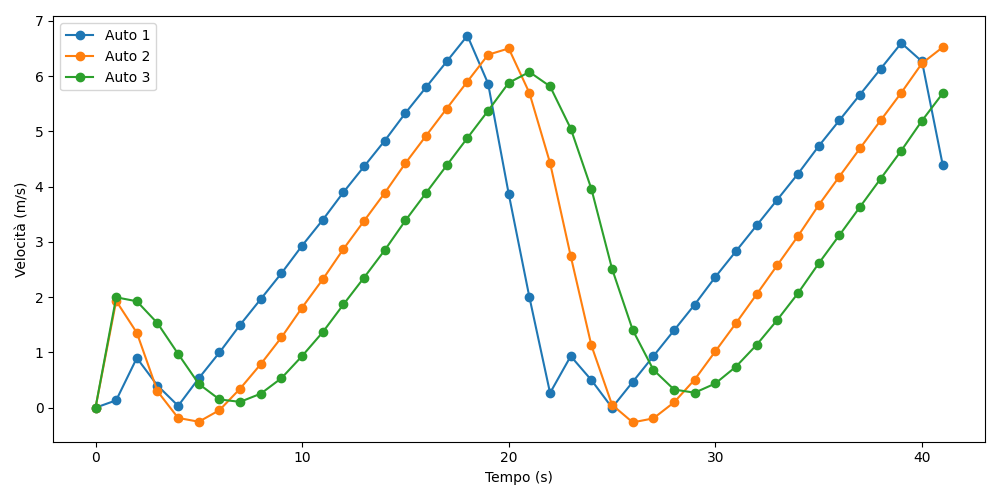
\includegraphics[width=0.96\textwidth]{images/5-experiment/car-number/velocity_3.png}
    \caption{Velocità con 3 auto.}
    \label{fig:3-cars-velocity}
\end{figure}
\vspace*{\fill}
\newpage
\vspace*{\fill}
\begin{table}[h]
    \centering
    \begin{tabular}{|c|c|c|c|}
        \hline
        N° auto & Distanza Iniziale & Distanza Target & Ritardo \\
        \hline
        $8$ & $6.0 m$ & $5.0 m$ & $0.2 s$ \\
        \hline
        $Time\hspace{0.2em}Headway$ & $\tau$ & $K_p$ & $K_d$  \\
        \hline
        $0.5$ & $0.1$ & $0.2$ & $0.7$ \\
        \hline
    \end{tabular}
\end{table}

\begin{figure}[H]
    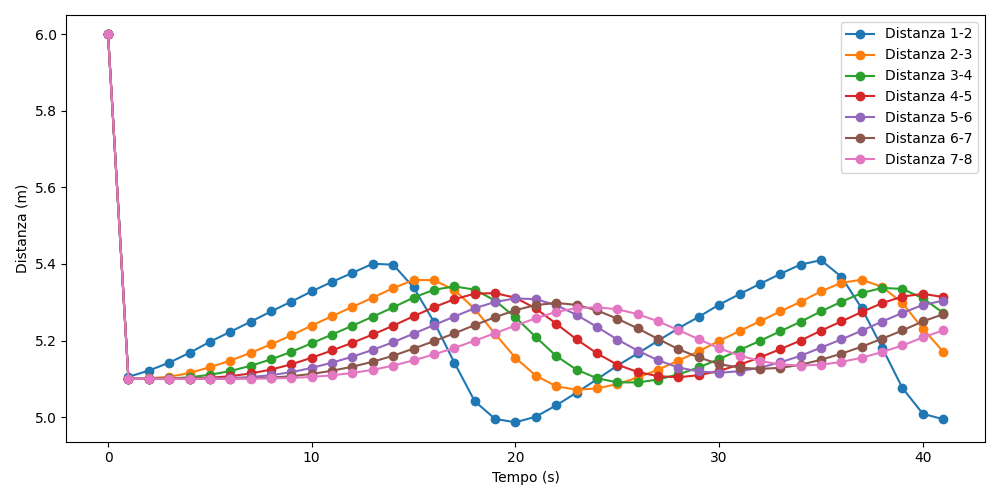
\includegraphics[width=0.96\textwidth]{images/5-experiment/car-number/distance_8.png}
    \caption{Distanze con 8 auto.}
    \label{fig:8-cars-distance}
\end{figure}

\begin{figure}[H]
    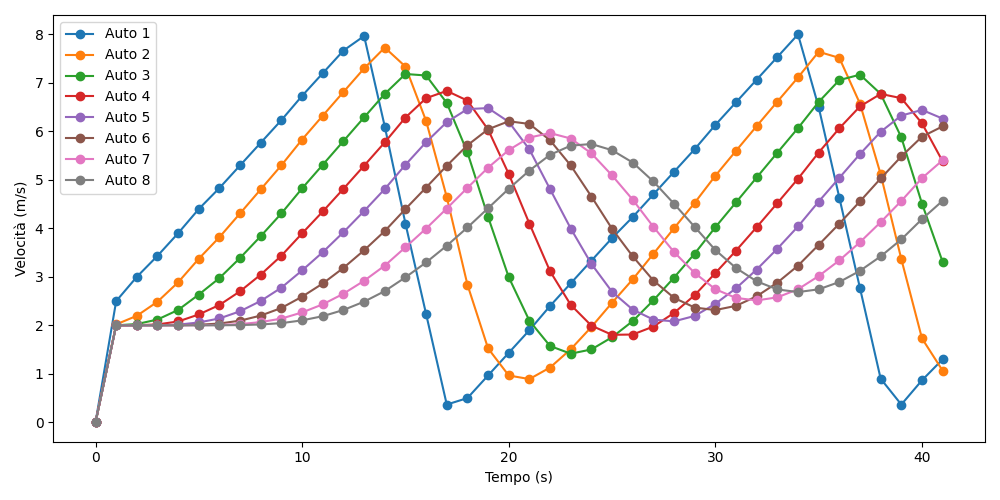
\includegraphics[width=0.96\textwidth]{images/5-experiment/car-number/velocity_8.png}
    \caption{Velocità con 8 auto.}
    \label{fig:8-cars-velocity}
\end{figure}
\vspace*{\fill}
\newpage
\vspace*{\fill}
\begin{table}[h]
    \centering
    \begin{tabular}{|c|c|c|c|}
        \hline
        N° auto & Distanza Iniziale & Distanza Target & Ritardo \\
        \hline
        $10$ & $6.0 m$ & $5.0 m$ & $0.2 s$ \\
        \hline
        $Time\hspace{0.2em}Headway$ & $\tau$ & $K_p$ & $K_d$  \\
        \hline
        $0.5$ & $0.1$ & $0.2$ & $0.7$ \\
        \hline
    \end{tabular}
\end{table}

\begin{figure}[H]
    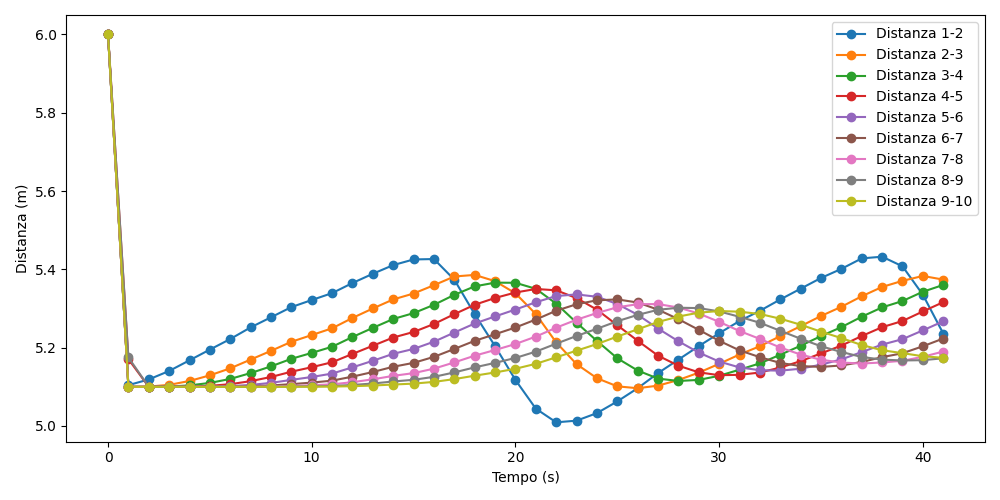
\includegraphics[width=0.96\textwidth]{images/5-experiment/car-number/distance_10.png}
    \caption{Distanze con 10 auto.}
    \label{fig:10-cars-distance}
\end{figure}

\begin{figure}[H]
    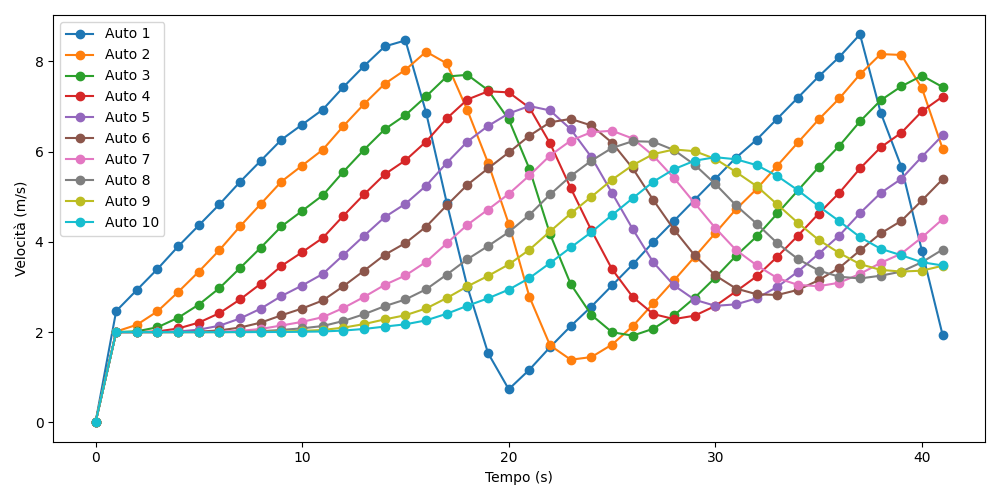
\includegraphics[width=0.96\textwidth]{images/5-experiment/car-number/velocity_10.png}
    \caption{Velocità con 10 auto.}
    \label{fig:10-cars-velocity}
\end{figure}

\vspace*{\fill}
\newpage

% CAR SPACING %

\subsubsection{Spazio tra le auto}
\vspace*{\fill}
\begin{table}[h]
    \centering
    \begin{tabular}{|c|c|c|c|}
        \hline
        N° auto & Distanza Iniziale & Distanza Target & Ritardo \\
        \hline
        $6$ & $2.0 m$ & $5.0 m$ & $0.2 s$ \\
        \hline
        $Time\hspace{0.2em}Headway$ & $\tau$ & $K_p$ & $K_d$  \\
        \hline
        $0.5$ & $0.1$ & $0.2$ & $0.7$ \\
        \hline
    \end{tabular}
\end{table}

\begin{figure}[H]
    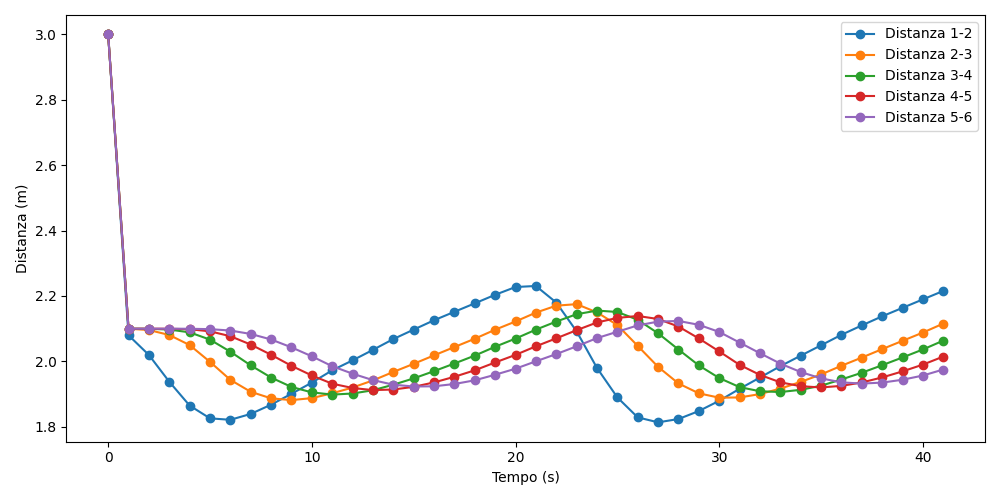
\includegraphics[width=0.96\textwidth]{images/5-experiment/car-spacing/distance_2.png}
    \caption{Distanze con $2.0 m$ come distanza iniziale.}
    \label{fig:2-space-distance}
\end{figure}

\begin{figure}[H]
    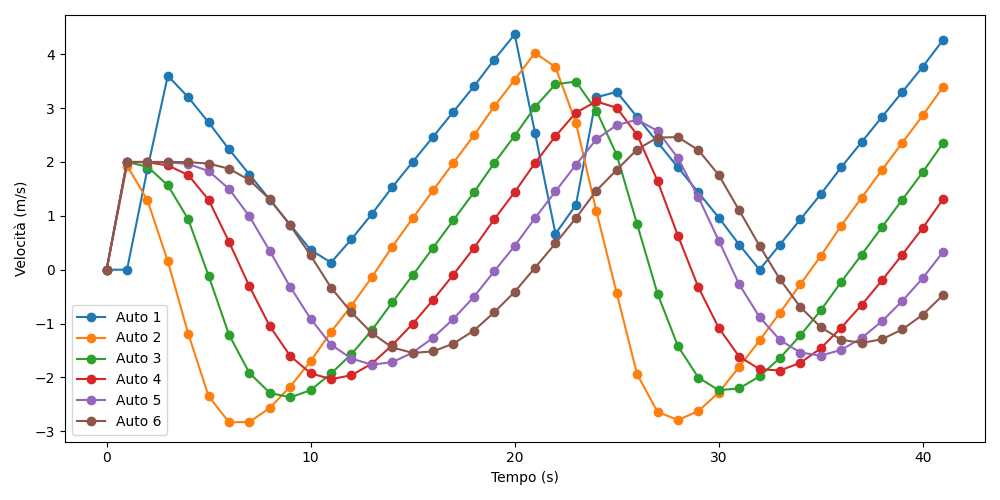
\includegraphics[width=0.96\textwidth]{images/5-experiment/car-spacing/velocity_2.png}
    \caption{Velocità con distanza iniziale $2.0 m$.}
    \label{fig:2-space-velocity}
\end{figure}
\vspace*{\fill}
\newpage
\vspace*{\fill}
\begin{table}[h]
    \centering
    \begin{tabular}{|c|c|c|c|}
        \hline
        N° auto & Distanza Iniziale & Distanza Target & Ritardo \\
        \hline
        $6$ & $10.0 m$ & $5.0 m$ & $0.2 s$ \\
        \hline
        $Time\hspace{0.2em}Headway$ & $\tau$ & $K_p$ & $K_d$  \\
        \hline
        $0.5$ & $0.1$ & $0.2$ & $0.7$ \\
        \hline
    \end{tabular}
\end{table}
\begin{figure}[H]
    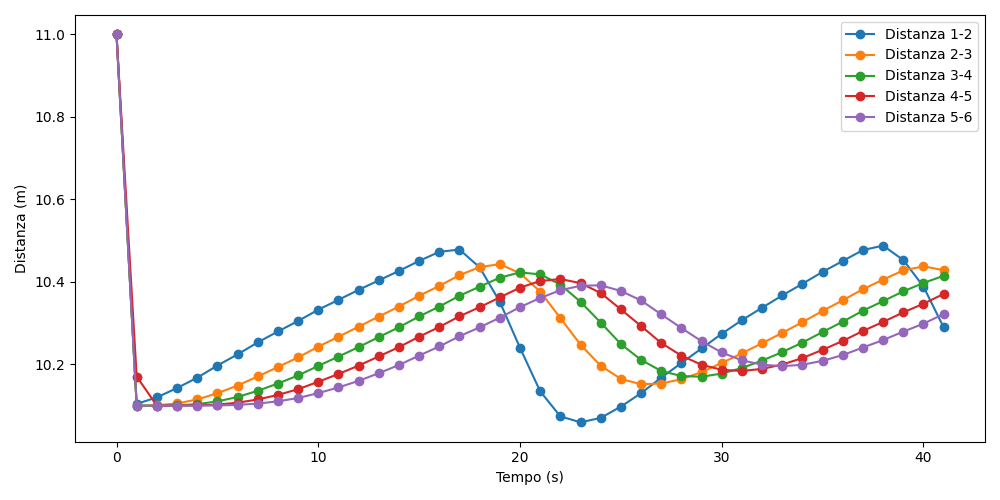
\includegraphics[width=0.96\textwidth]{images/5-experiment/car-spacing/distance_10.png}
    \caption{Distanze con $10.0 m$ come distanza iniziale.}
    \label{fig:10-space-distance}
\end{figure}

\begin{figure}[H]
    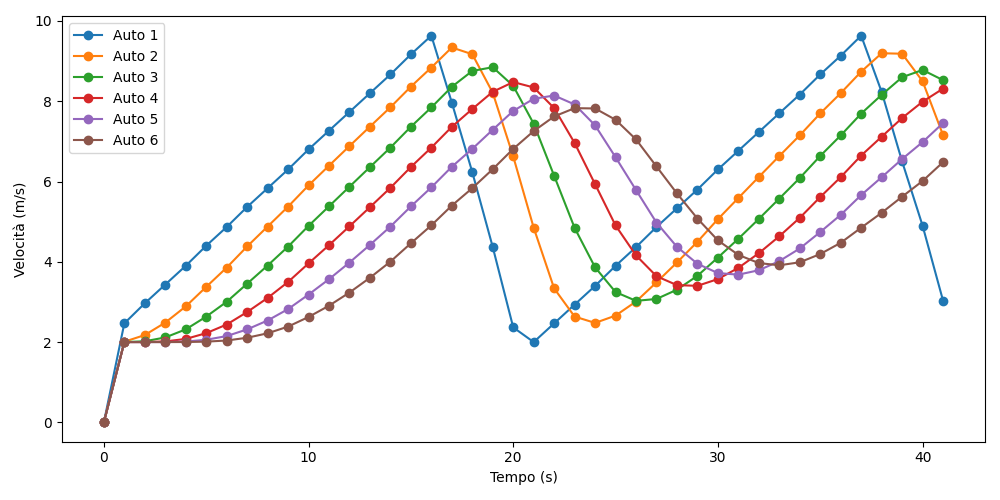
\includegraphics[width=0.96\textwidth]{images/5-experiment/car-spacing/velocity_10.png}
    \caption{Velocità con distanza iniziale $10.0 m$.}
    \label{fig:10-space-velocity}
\end{figure}
\vspace*{\fill}
\newpage
\vspace*{\fill}
\begin{table}[h]
    \centering
    \begin{tabular}{|c|c|c|c|}
        \hline
        N° auto & Distanza Iniziale & Distanza Target & Ritardo \\
        \hline
        $6$ & $20.0 m$ & $5.0 m$ & $0.2 s$ \\
        \hline
        $Time\hspace{0.2em}Headway$ & $\tau$ & $K_p$ & $K_d$  \\
        \hline
        $0.5$ & $0.1$ & $0.2$ & $0.7$ \\
        \hline
    \end{tabular}
\end{table}

\begin{figure}[H]
    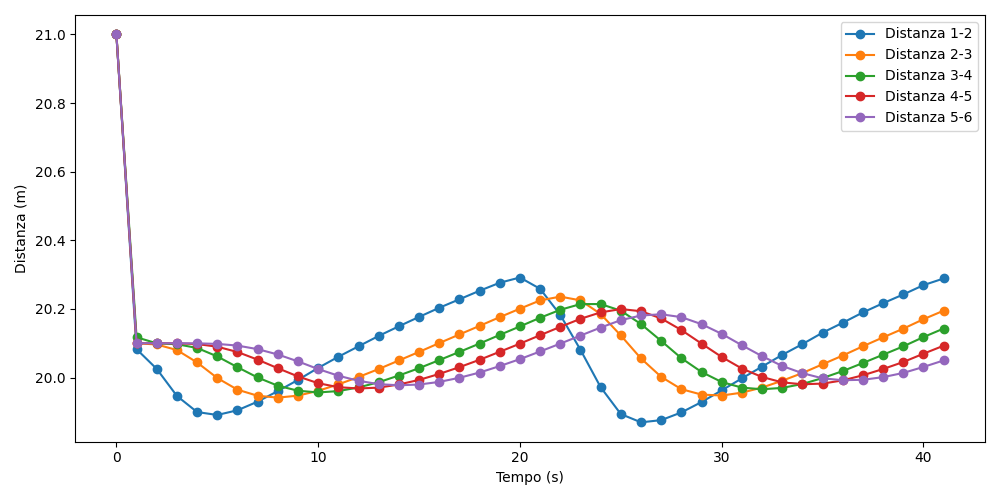
\includegraphics[width=0.96\textwidth]{images/5-experiment/car-spacing/distance_20.png}
    \caption{Distanze con $20.0 m$ come distanza iniziale.}
    \label{fig:20-space-distance}
\end{figure}

\begin{figure}[H]
    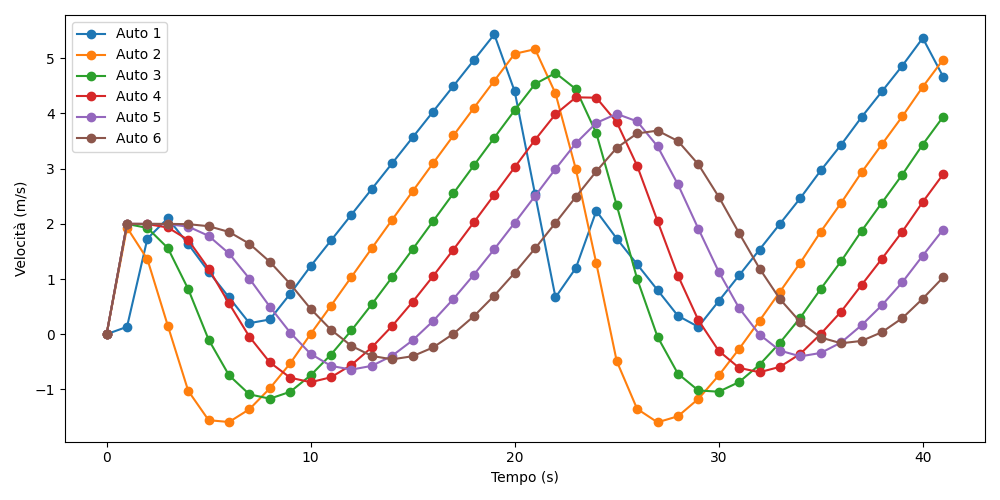
\includegraphics[width=0.96\textwidth]{images/5-experiment/car-spacing/velocity_20.png}
    \caption{Velocità con distanza iniziale $20.0 m$.}
    \label{fig:20-space-velocity}
\end{figure}
\vspace*{\fill}
\newpage

% DELAY %

\subsubsection{Ritardo di comunicazione}
\vspace*{\fill}
\begin{table}[h]
    \centering
    \begin{tabular}{|c|c|c|c|}
        \hline
        N° auto & Distanza Iniziale & Distanza Target & Ritardo \\
        \hline
        $6$ & $6.0 m$ & $5.0 m$ & $0.5 s$ \\
        \hline
        $Time\hspace{0.2em}Headway$ & $\tau$ & $K_p$ & $K_d$  \\
        \hline
        $0.5$ & $0.1$ & $0.2$ & $0.7$ \\
        \hline
    \end{tabular}
\end{table}

\begin{figure}[H]
    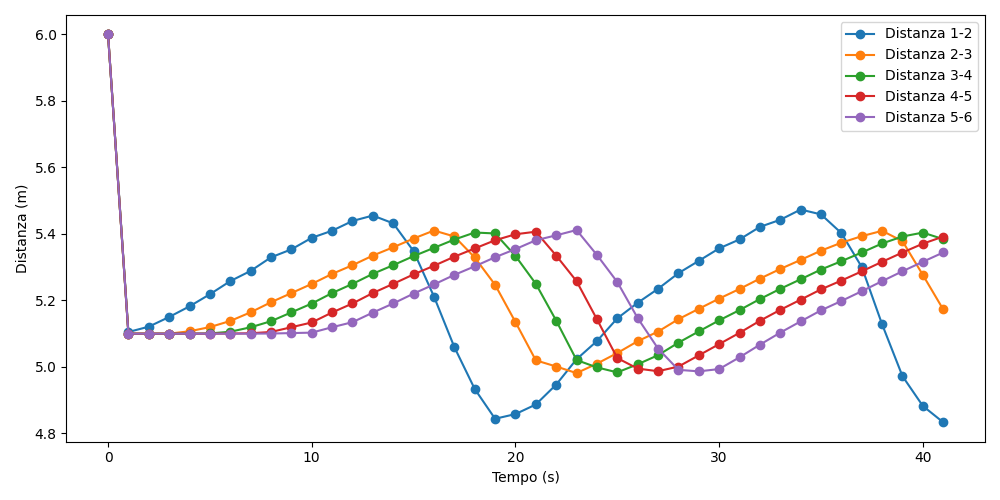
\includegraphics[width=0.96\textwidth]{images/5-experiment/delay/distance_0,5.png}
    \caption{Distanze con ritardo a $0.5 s$.}
    \label{fig:0.5-delay-distance}
\end{figure}

\begin{figure}[H]
    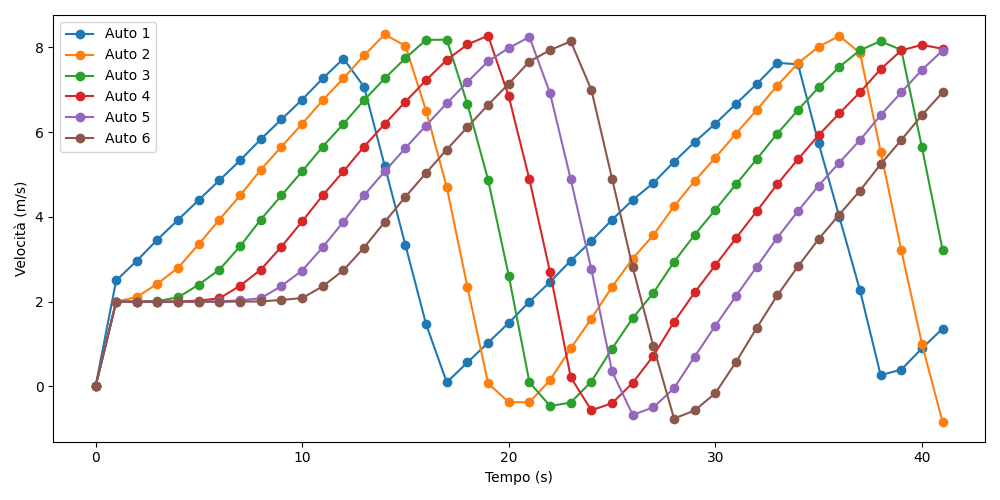
\includegraphics[width=0.96\textwidth]{images/5-experiment/delay/velocity_0,5.png}
    \caption{Velocità con ritardo a $0.5 s$.}
    \label{fig:0.5-delay-velocity}
\end{figure}
\vspace*{\fill}
\newpage
\vspace*{\fill}
\begin{table}[h]
    \centering
    \begin{tabular}{|c|c|c|c|}
        \hline
        N° auto & Distanza Iniziale & Distanza Target & Ritardo \\
        \hline
        $6$ & $6.0 m$ & $5.0 m$ & $1 s$ \\
        \hline
        $Time\hspace{0.2em}Headway$ & $\tau$ & $K_p$ & $K_d$  \\
        \hline
        $0.5$ & $0.1$ & $0.2$ & $0.7$ \\
        \hline
    \end{tabular}
\end{table}

\begin{figure}[H]
    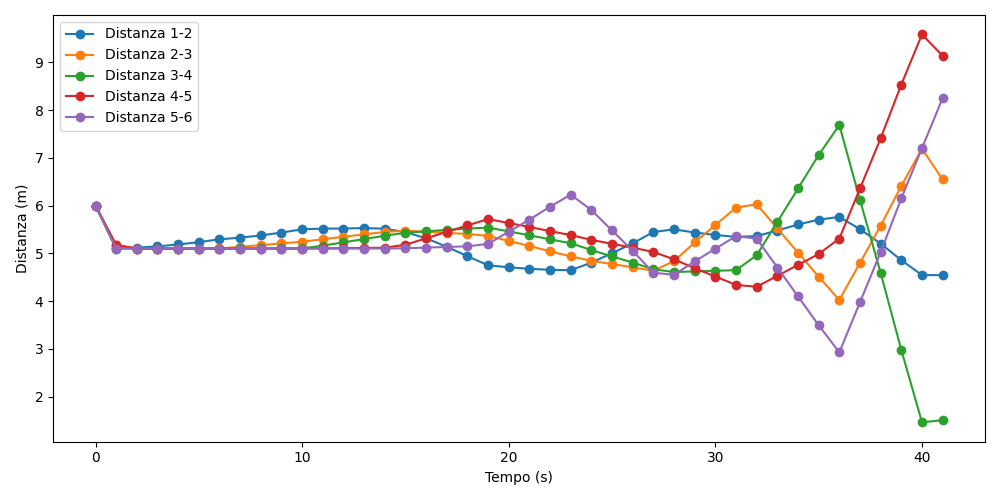
\includegraphics[width=0.96\textwidth]{images/5-experiment/delay/distance_1.png}
    \caption{Distanze con ritardo a $1 s$.}
    \label{fig:1-delay-distance}
\end{figure}

\begin{figure}[H]
    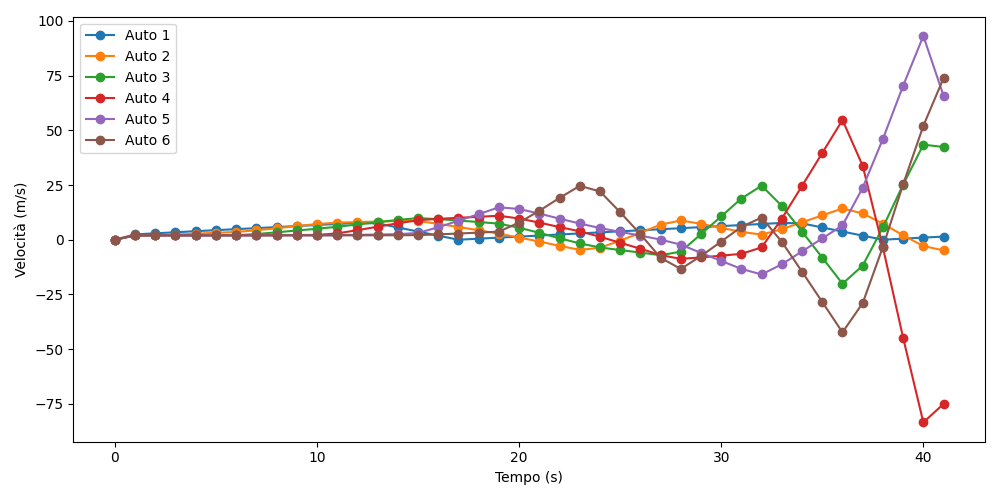
\includegraphics[width=0.96\textwidth]{images/5-experiment/delay/velocity_1.png}
    \caption{Velocità con ritardo a $1 s$.}
    \label{fig:1-delay-velocity}
\end{figure}
\vspace*{\fill}
\newpage

% TIME HEADWAY %

\subsubsection{Time Headway}
\vspace*{\fill}
\begin{table}[h]
    \centering
    \begin{tabular}{|c|c|c|c|}
        \hline
        N° auto & Distanza Iniziale & Distanza Target & Ritardo \\
        \hline
        $6$ & $6.0 m$ & $5.0 m$ & $0.2 s$ \\
        \hline
        $Time\hspace{0.2em}Headway$ & $\tau$ & $K_p$ & $K_d$  \\
        \hline
        $0.05$ & $0.1$ & $0.2$ & $0.7$ \\
        \hline
    \end{tabular}
\end{table}

\begin{figure}[H]
    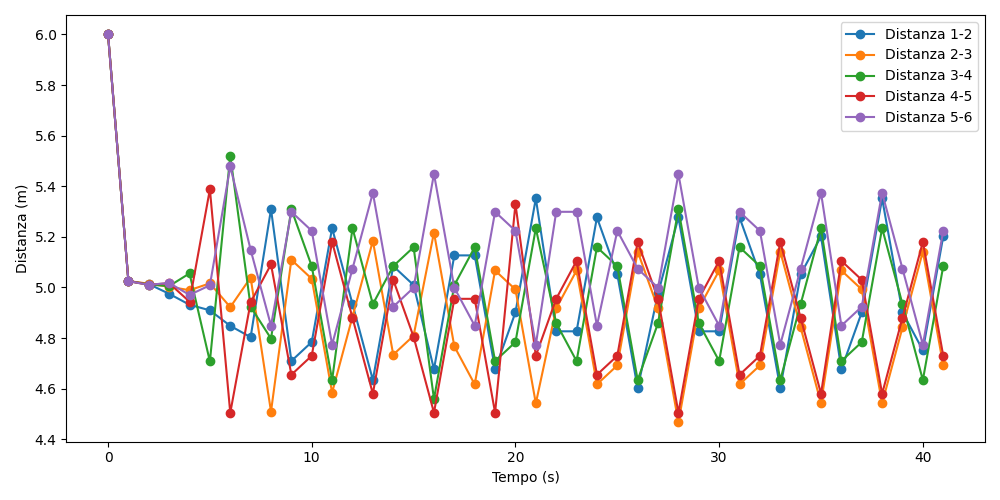
\includegraphics[width=0.96\textwidth]{images/5-experiment/time-headway/distance_0,05.png}
    \caption{Distanze con $Time\hspace{0.2em}Headway$ a $0.05$.}
    \label{fig:0.05-headway-distance}
\end{figure}

\begin{figure}[H]
    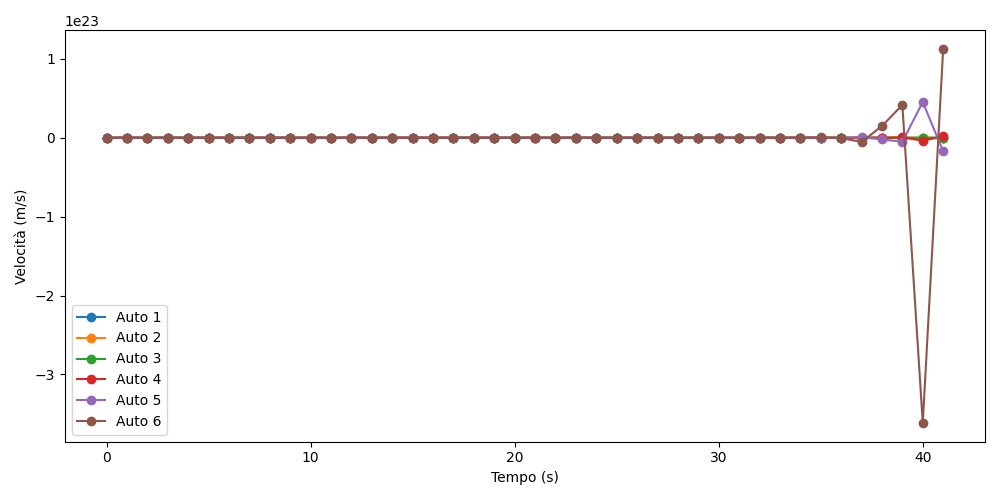
\includegraphics[width=0.96\textwidth]{images/5-experiment/time-headway/velocity_0,05.png}
    \caption{Velocità con $Time\hspace{0.2em}Headway$ a $0.05$.}
    \label{fig:0.05-headway-velocity}
\end{figure}
\vspace*{\fill}
\newpage
\vspace*{\fill}
\begin{table}[h]
    \centering
    \begin{tabular}{|c|c|c|c|}
        \hline
        N° auto & Distanza Iniziale & Distanza Target & Ritardo \\
        \hline
        $6$ & $6.0 m$ & $5.0 m$ & $0.2 s$ \\
        \hline
        $Time\hspace{0.2em}Headway$ & $\tau$ & $K_p$ & $K_d$  \\
        \hline
        $0.1$ & $0.1$ & $0.2$ & $0.7$ \\
        \hline
    \end{tabular}
\end{table}

\begin{figure}[H]
    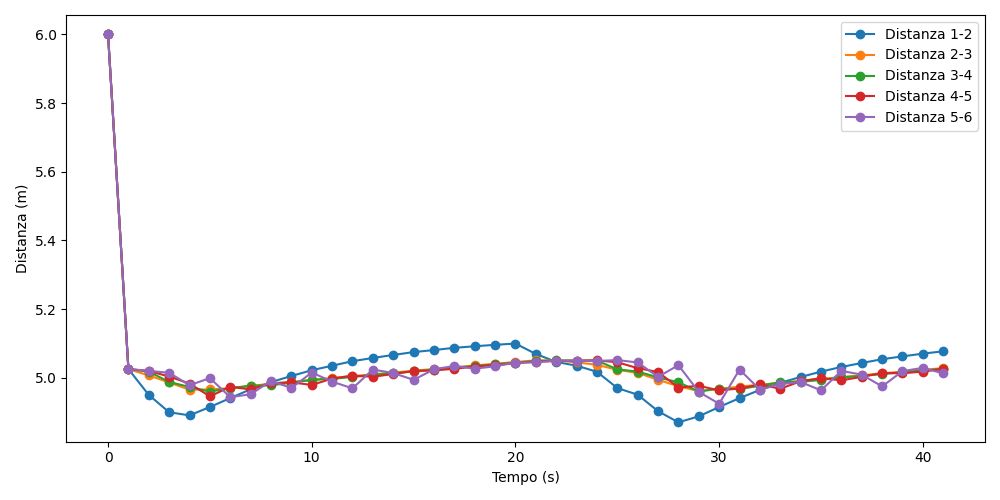
\includegraphics[width=0.96\textwidth]{images/5-experiment/time-headway/distance_0,1.png}
    \caption{Distanze con $Time\hspace{0.2em}Headway$ a $0.1$.}
    \label{fig:0.1-headway-distance}
\end{figure}

\begin{figure}[H]
    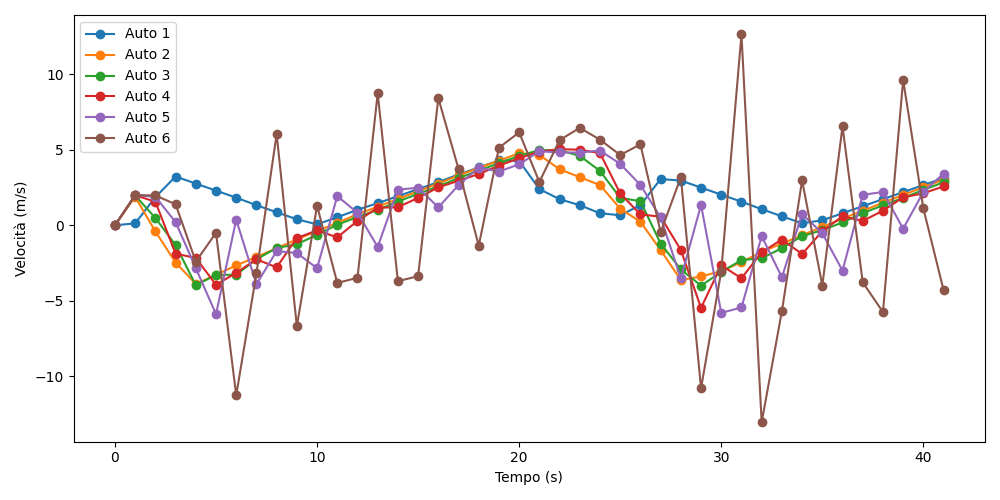
\includegraphics[width=0.96\textwidth]{images/5-experiment/time-headway/velocity_0,1.png}
    \caption{Velocità con $Time\hspace{0.2em}Headway$ a $0.1$.}
    \label{fig:0.1-headway-velocity}
\end{figure}
\vspace*{\fill}
\newpage
\vspace*{\fill}
\begin{table}[h]
    \centering
    \begin{tabular}{|c|c|c|c|}
        \hline
        N° auto & Distanza Iniziale & Distanza Target & Ritardo \\
        \hline
        $6$ & $6.0 m$ & $5.0 m$ & $0.2 s$ \\
        \hline
        $Time\hspace{0.2em}Headway$ & $\tau$ & $K_p$ & $K_d$  \\
        \hline
        $1$ & $0.1$ & $0.2$ & $0.7$ \\
        \hline
    \end{tabular}
\end{table}

\begin{figure}[H]
    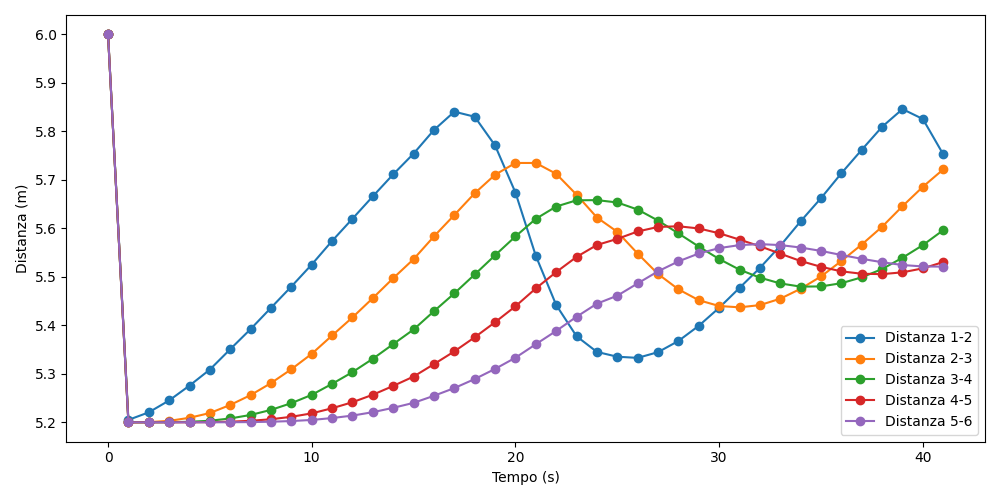
\includegraphics[width=0.96\textwidth]{images/5-experiment/time-headway/distance_1.png}
    \caption{Distanze con $Time\hspace{0.2em}Headway$ a $1$.}
    \label{fig:1-headway-distance}
\end{figure}

\begin{figure}[H]
    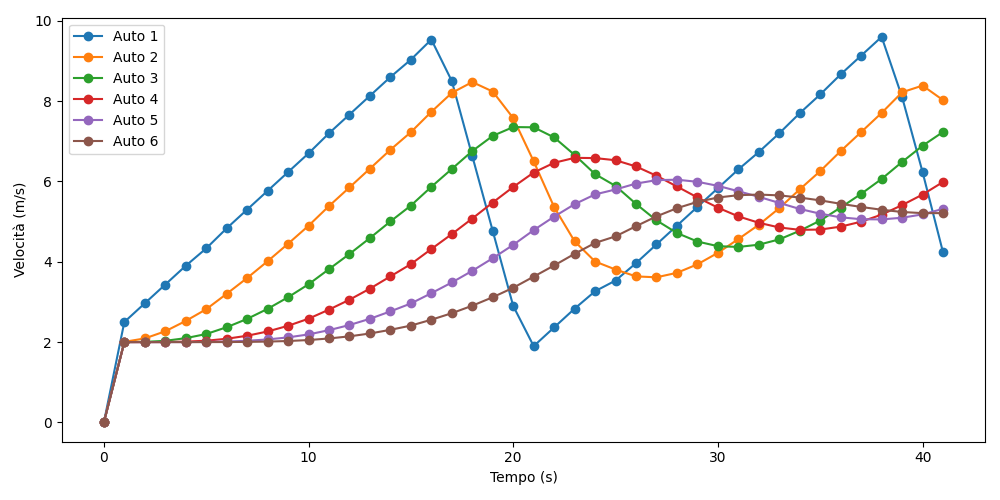
\includegraphics[width=0.96\textwidth]{images/5-experiment/time-headway/velocity_1.png}
    \caption{Velocità con $Time\hspace{0.2em}Headway$ a $1$.}
    \label{fig:1-headway-velocity}
\end{figure}
\vspace*{\fill}
\newpage
\vspace*{\fill}
\begin{table}[h]
    \centering
    \begin{tabular}{|c|c|c|c|}
        \hline
        N° auto & Distanza Iniziale & Distanza Target & Ritardo \\
        \hline
        $6$ & $6.0 m$ & $5.0 m$ & $0.2 s$ \\
        \hline
        $Time\hspace{0.2em}Headway$ & $\tau$ & $K_p$ & $K_d$  \\
        \hline
        $2$ & $0.1$ & $0.2$ & $0.7$ \\
        \hline
    \end{tabular}
\end{table}

\begin{figure}[H]
    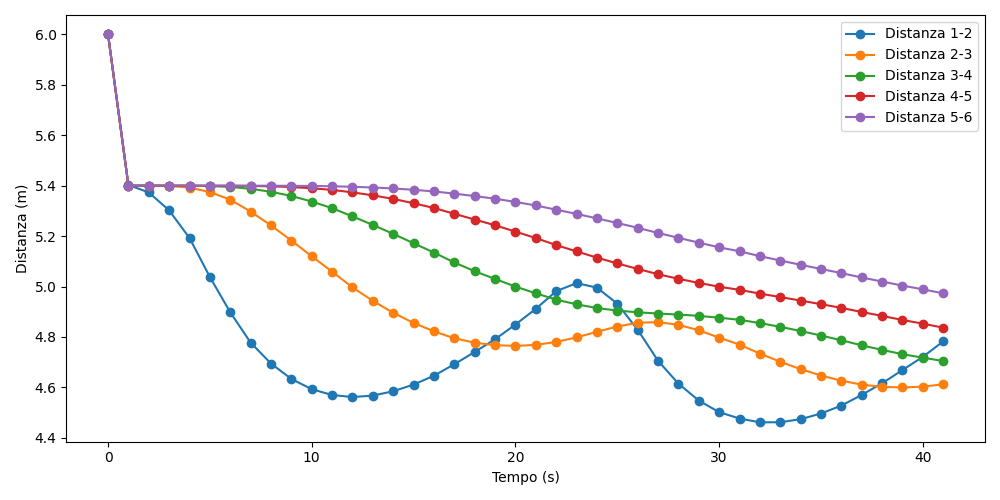
\includegraphics[width=0.96\textwidth]{images/5-experiment/time-headway/distance_2.png}
    \caption{Distanze con $Time\hspace{0.2em}Headway$ a $2$.}
    \label{fig:2-headway-distance}
\end{figure}

\begin{figure}[H]
    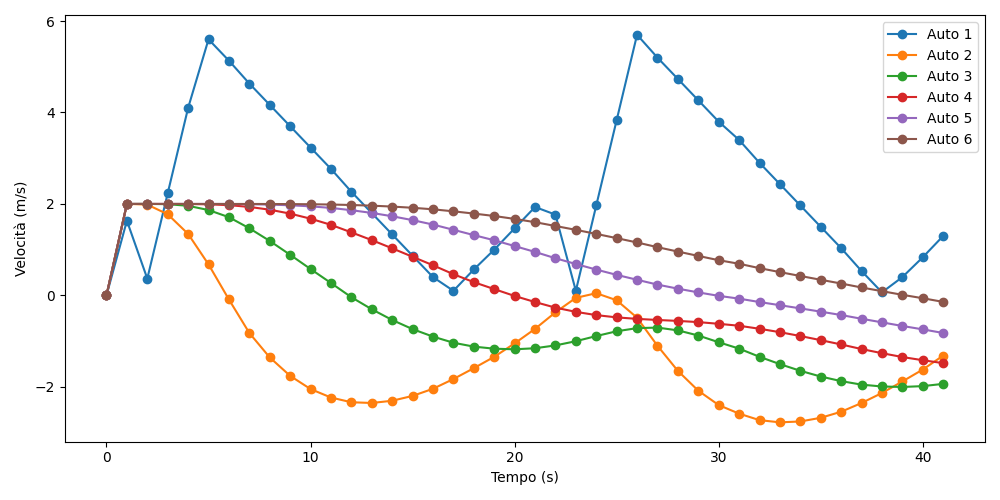
\includegraphics[width=0.96\textwidth]{images/5-experiment/time-headway/velocity_2.png}
    \caption{Velocità con $Time\hspace{0.2em}Headway$ a $2$.}
    \label{fig:2-headway-velocity}
\end{figure}
\vspace*{\fill}
\newpage

% TAU %

\subsubsection{Tau \texorpdfstring{($\tau$)}{}}
\vspace*{\fill}
\begin{table}[h]
    \centering
    \begin{tabular}{|c|c|c|c|}
        \hline
        N° auto & Distanza Iniziale & Distanza Target & Ritardo \\
        \hline
        $6$ & $6.0 m$ & $5.0 m$ & $0.2 s$ \\
        \hline
        $Time\hspace{0.2em}Headway$ & $\tau$ & $K_p$ & $K_d$  \\
        \hline
        $0.5$ & $0.01$ & $0.2$ & $0.7$ \\
        \hline
    \end{tabular}
\end{table}

\begin{figure}[H]
    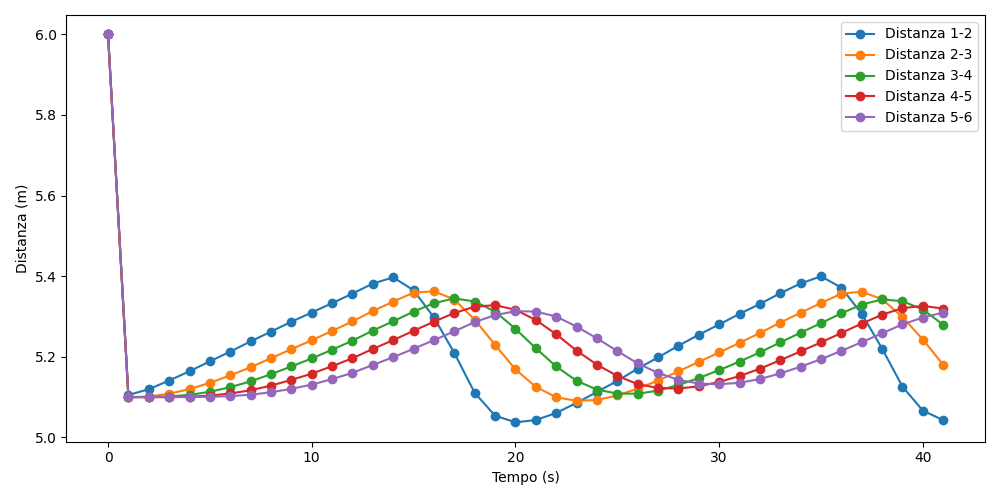
\includegraphics[width=0.96\textwidth]{images/5-experiment/tau/distance_0,01.png}
    \caption{Distanze con $\tau$ a $0.01$.}
    \label{fig:0.01-tau-distance}
\end{figure}

\begin{figure}[H]
    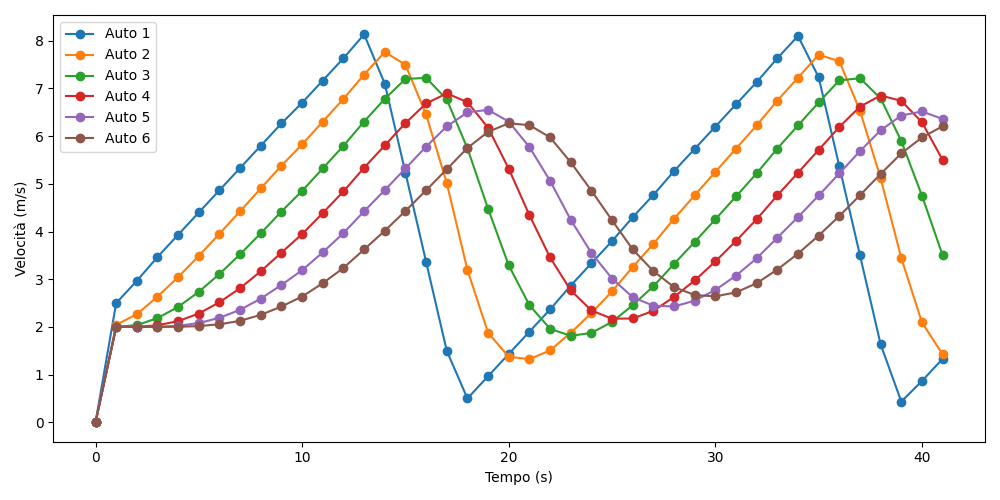
\includegraphics[width=0.96\textwidth]{images/5-experiment/tau/velocity_0,01.png}
    \caption{Velocità con $\tau$ a $0.01$.}
    \label{fig:0.01-tau-velocity}
\end{figure}
\vspace*{\fill}
\newpage
\vspace*{\fill}
\begin{table}[h]
    \centering
    \begin{tabular}{|c|c|c|c|}
        \hline
        N° auto & Distanza Iniziale & Distanza Target & Ritardo \\
        \hline
        $6$ & $6.0 m$ & $5.0 m$ & $0.2 s$ \\
        \hline
        $Time\hspace{0.2em}Headway$ & $\tau$ & $K_p$ & $K_d$  \\
        \hline
        $0.5$ & $0.7$ & $0.2$ & $0.7$ \\
        \hline
    \end{tabular}
\end{table}
\begin{figure}[H]
    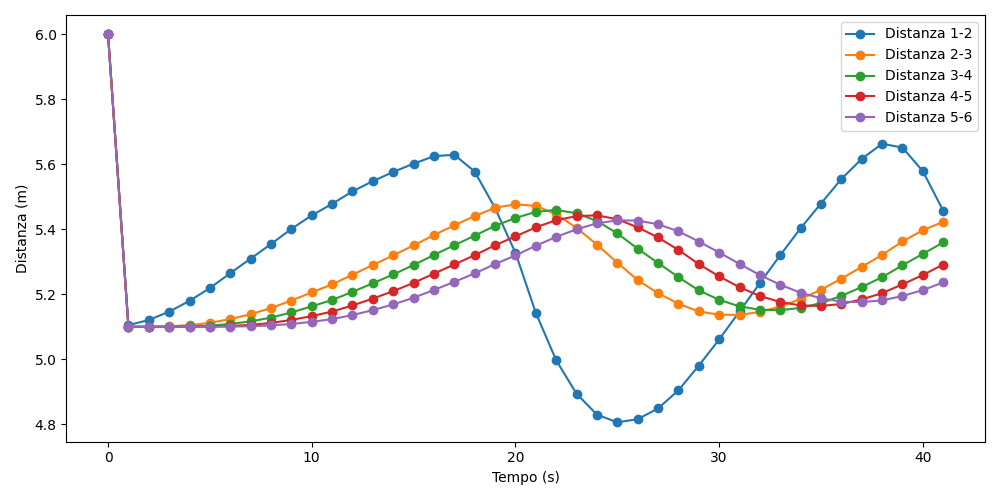
\includegraphics[width=0.96\textwidth]{images/5-experiment/tau/distance_0,7.png}
    \caption{Distanze con $\tau$ a $0.7$.}
    \label{fig:0.7-tau-distance}
\end{figure}

\begin{figure}[H]
    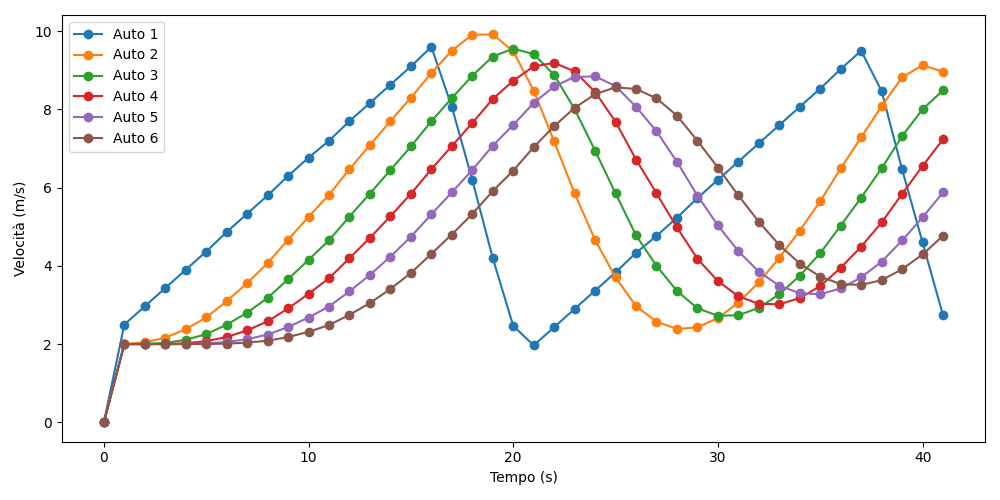
\includegraphics[width=0.96\textwidth]{images/5-experiment/tau/velocity_0,7.png}
    \caption{Velocità con $\tau$ a $0.7$.}
    \label{fig:0.7-tau-velocity}
\end{figure}
\vspace*{\fill}
\newpage
\vspace*{\fill}
\begin{table}[h]
    \centering
    \begin{tabular}{|c|c|c|c|}
        \hline
        N° auto & Distanza Iniziale & Distanza Target & Ritardo \\
        \hline
        $6$ & $6.0 m$ & $5.0 m$ & $0.2 s$ \\
        \hline
        $Time\hspace{0.2em}Headway$ & $\tau$ & $K_p$ & $K_d$  \\
        \hline
        $0.5$ & $2.0$ & $0.2$ & $0.7$ \\
        \hline
    \end{tabular}
\end{table}

\begin{figure}[H]
    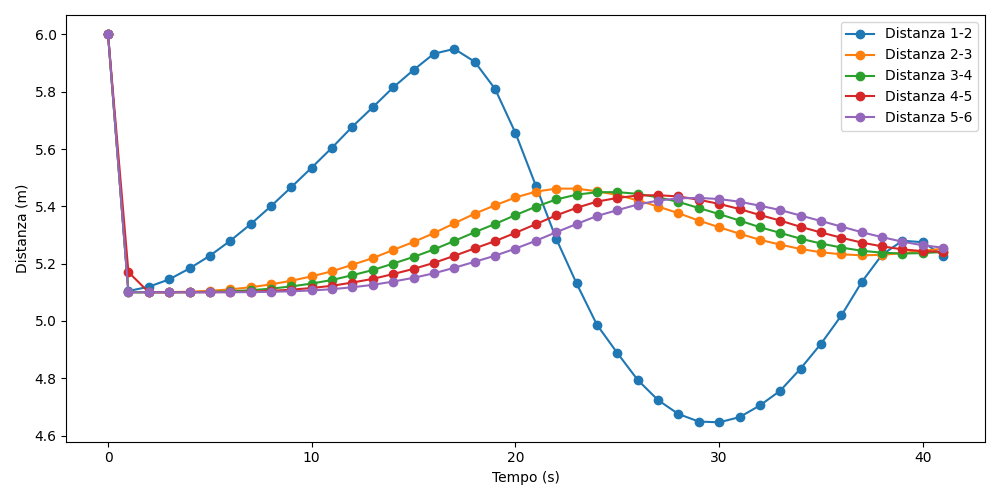
\includegraphics[width=0.96\textwidth]{images/5-experiment/tau/distance_2.png}
    \caption{Distanze con $\tau$ a $2.0$.}
    \label{fig:2-tau-distance}
\end{figure}

\begin{figure}[H]
    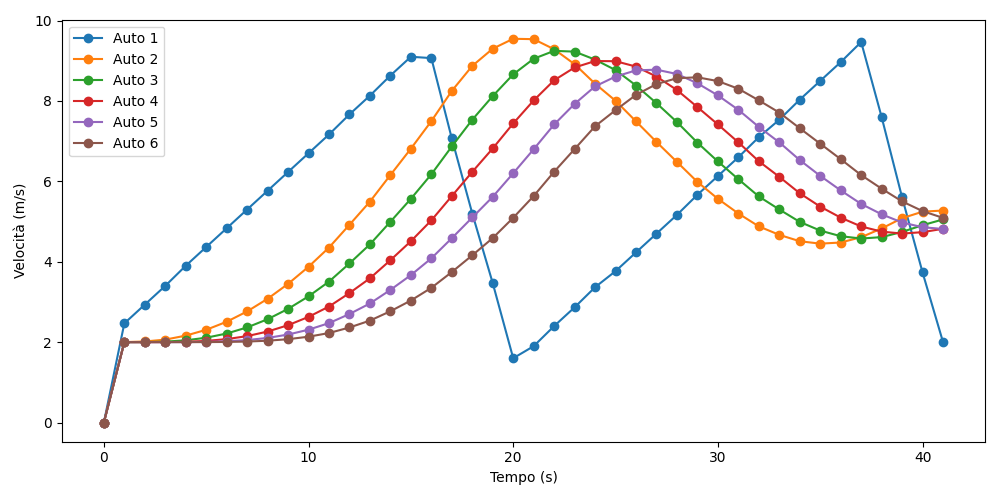
\includegraphics[width=0.96\textwidth]{images/5-experiment/tau/velocity_2.png}
    \caption{Velocità con $\tau$ a $2.0$.}
    \label{fig:2-tau-velocity}
\end{figure}
\vspace*{\fill}
\newpage


% VELOCITÀ CON PARAMETRI DEFAULT %

\subsubsection{Velocità con parametri di default}

\begin{table}[h]
    \centering
    \begin{tabular}{|c|c|c|c|c|}
        \hline
        Velocità $t1$ & Velocità $t2$ & Velocità $t3$ &Velocità $t4$ &Velocità $t5$\\
        \hline
            $0\hspace{0.2em}m/s$ & $0\hspace{0.2em}m/s$ & $0\hspace{0.2em}m/s$ & $0\hspace{0.2em}m/s$ & $0\hspace{0.2em}m/s$ \\
        \hline
    \end{tabular}
\end{table}
\begin{table}[h]
    \centering
    \begin{tabular}{|c|c|c|c|}
        \hline
        N° auto & Distanza Iniziale & Distanza Target & Ritardo \\
        \hline
        $6$ & $6.0 m$ & $5.0 m$ & $0.2 s$ \\
        \hline
        $Time\hspace{0.2em}Headway$ & $\tau$ & $K_p$ & $K_d$  \\
        \hline
        $0.5$ & $0.1$ & $0.2$ & $0.7$ \\
        \hline
    \end{tabular}
\end{table}

\begin{figure}[H]
    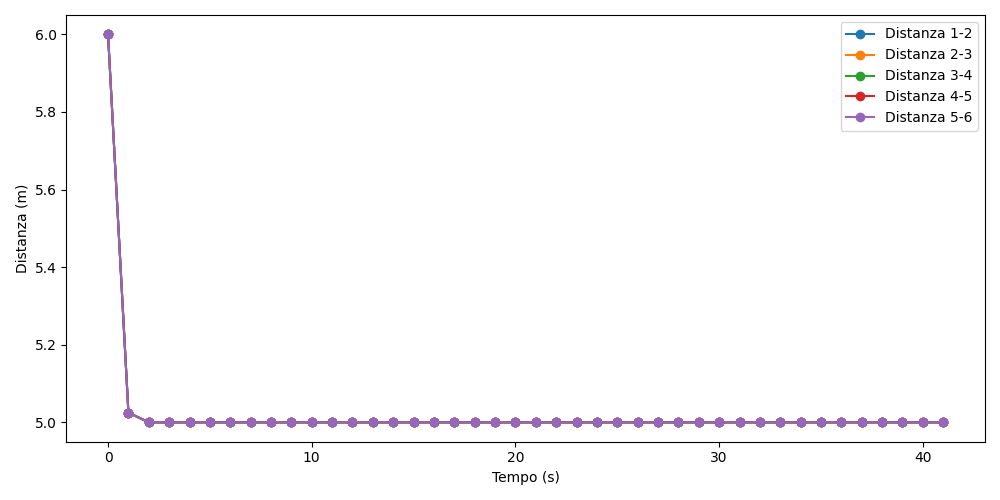
\includegraphics[width=0.96\textwidth]{images/5-experiment/velocity/distance_0-0-0-0-0.png}
    \caption{Distanze con primo veicolo fermo.}
    \label{fig:0-constvelocity-distance}
\end{figure}

\begin{figure}[H]
    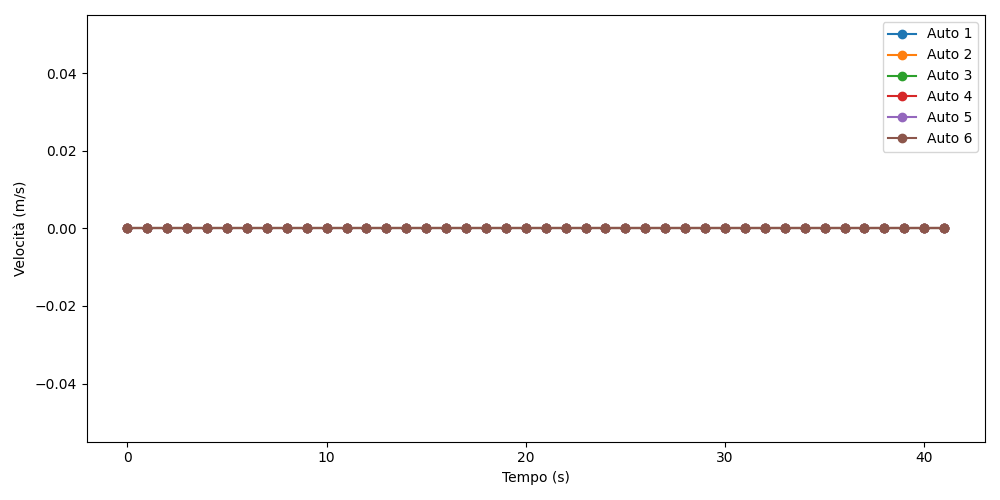
\includegraphics[width=0.96\textwidth]{images/5-experiment/velocity/velocity_0-0-0-0-0.png}
    \caption{Velocità con primo veicolo fermo.}
    \label{fig:0-constvelocity-velocity}
\end{figure}

\newpage

\begin{table}[h]
    \centering
    \begin{tabular}{|c|c|c|c|c|}
        \hline
        Velocità $t1$ & Velocità $t2$ & Velocità $t3$ &Velocità $t4$ &Velocità $t5$\\
        \hline
            $10\hspace{0.2em}m/s$ & $10\hspace{0.2em}m/s$ & $10\hspace{0.2em}m/s$ & $10\hspace{0.2em}m/s$ & $10\hspace{0.2em}m/s$ \\
        \hline
    \end{tabular}
\end{table}
\begin{table}[h]
    \centering
    \begin{tabular}{|c|c|c|c|}
        \hline
        N° auto & Distanza Iniziale & Distanza Target & Ritardo \\
        \hline
        $6$ & $6.0 m$ & $5.0 m$ & $0.2 s$ \\
        \hline
        $Time\hspace{0.2em}Headway$ & $\tau$ & $K_p$ & $K_d$  \\
        \hline
        $0.5$ & $0.1$ & $0.2$ & $0.7$ \\
        \hline
    \end{tabular}
\end{table}

\begin{figure}[H]
    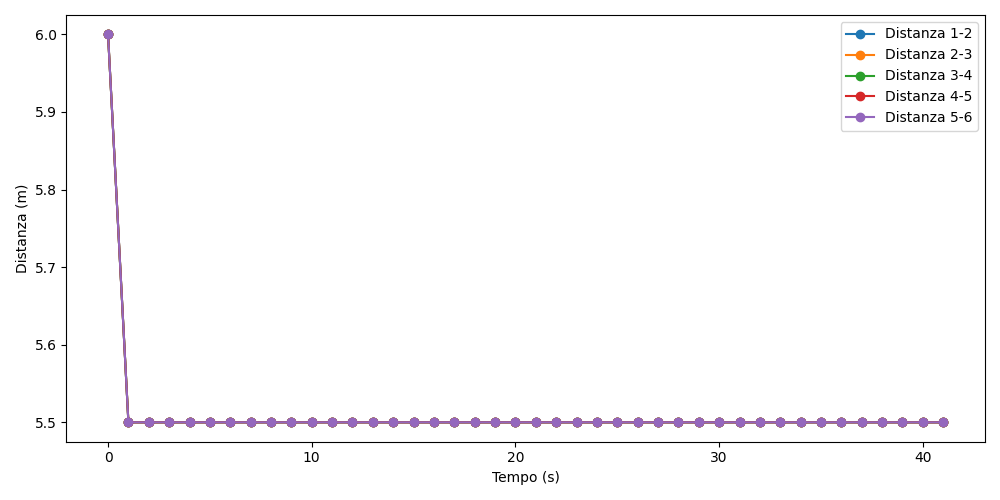
\includegraphics[width=0.96\textwidth]{images/5-experiment/velocity/distance_10-10-10-10-10.png}
    \caption{Distanze con velocità costante a $10\hspace{0.2em}m/s$.}
    \label{fig:10-constvelocity-distance}
\end{figure}

\begin{figure}[H]
    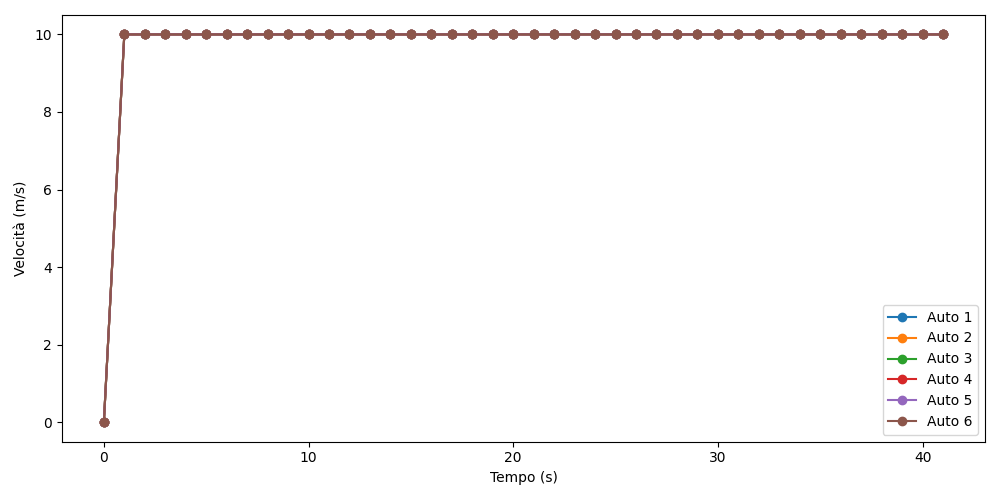
\includegraphics[width=0.96\textwidth]{images/5-experiment/velocity/velocity_10-10-10-10-10.png}
    \caption{Velocità con velocità costante a $10\hspace{0.2em}m/s$.}
    \label{fig:10-constvelocity-velocity}
\end{figure}

\newpage

\begin{table}[h]
    \centering
    \begin{tabular}{|c|c|c|c|c|}
        \hline
        Velocità $t1$ & Velocità $t2$ & Velocità $t3$ &Velocità $t4$ &Velocità $t5$\\
        \hline
            $35\hspace{0.2em}m/s$ & $35\hspace{0.2em}m/s$ & $35\hspace{0.2em}m/s$ & $35\hspace{0.2em}m/s$ & $35\hspace{0.2em}m/s$ \\
        \hline
    \end{tabular}
\end{table}
\begin{table}[h]
    \centering
    \begin{tabular}{|c|c|c|c|}
        \hline
        N° auto & Distanza Iniziale & Distanza Target & Ritardo \\
        \hline
        $6$ & $6.0 m$ & $5.0 m$ & $0.2 s$ \\
        \hline
        $Time\hspace{0.2em}Headway$ & $\tau$ & $K_p$ & $K_d$  \\
        \hline
        $0.5$ & $0.1$ & $0.2$ & $0.7$ \\
        \hline
    \end{tabular}
\end{table}

\begin{figure}[H]
    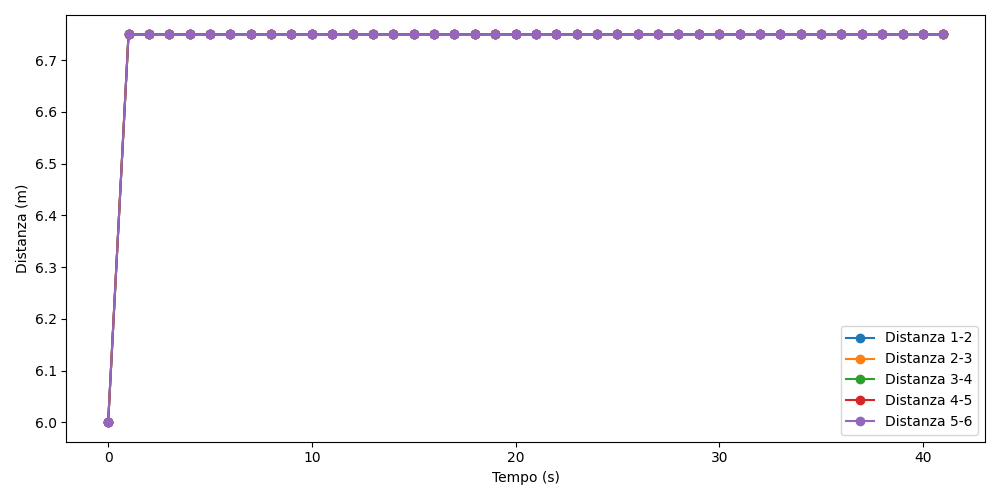
\includegraphics[width=0.96\textwidth]{images/5-experiment/velocity/distance_35-35-35-35-35.png}
    \caption{Distanze con velocità costante a $35\hspace{0.2em}m/s$.}
    \label{fig:35-constvelocity-distance}
\end{figure}

\begin{figure}[H]
    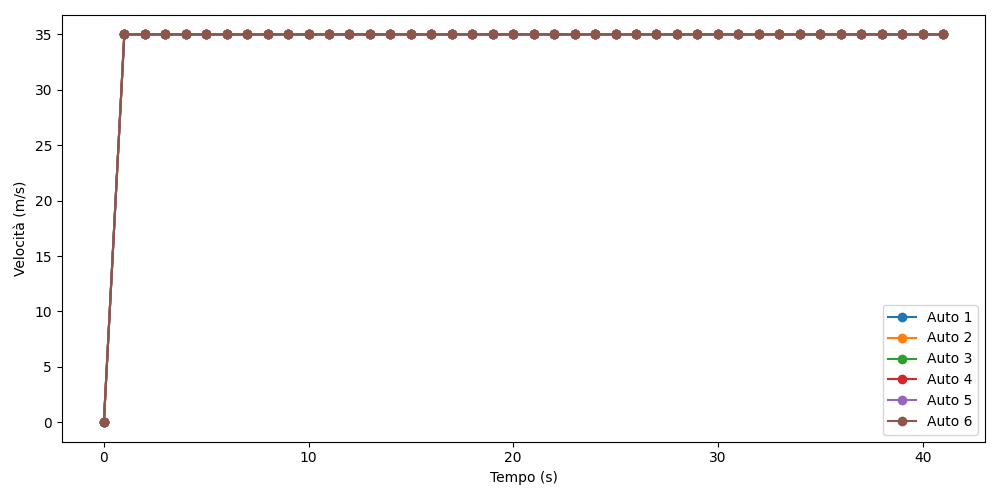
\includegraphics[width=0.96\textwidth]{images/5-experiment/velocity/velocity_35-35-35-35-35.png}
    \caption{Velocità con velocità costante a $35\hspace{0.2em}m/s$.}
    \label{fig:35-constvelocity-velocity}
\end{figure}

\newpage

\begin{table}[h]
    \centering
    \begin{tabular}{|c|c|c|c|c|}
        \hline
        Velocità $t1$ & Velocità $t2$ & Velocità $t3$ &Velocità $t4$ &Velocità $t5$\\
        \hline
            $20\hspace{0.2em}m/s$ & $0\hspace{0.2em}m/s$ & $20\hspace{0.2em}m/s$ & $0\hspace{0.2em}m/s$ & $20\hspace{0.2em}m/s$ \\
        \hline
    \end{tabular}
\end{table}
\begin{table}[h]
    \centering
    \begin{tabular}{|c|c|c|c|}
        \hline
        N° auto & Distanza Iniziale & Distanza Target & Ritardo \\
        \hline
        $6$ & $6.0 m$ & $5.0 m$ & $0.2 s$ \\
        \hline
        $Time\hspace{0.2em}Headway$ & $\tau$ & $K_p$ & $K_d$ \\
        \hline
        $0.5$ & $0.1$ & $0.2$ & $0.7$ \\
        \hline
    \end{tabular}
\end{table}

\begin{figure}[H]
    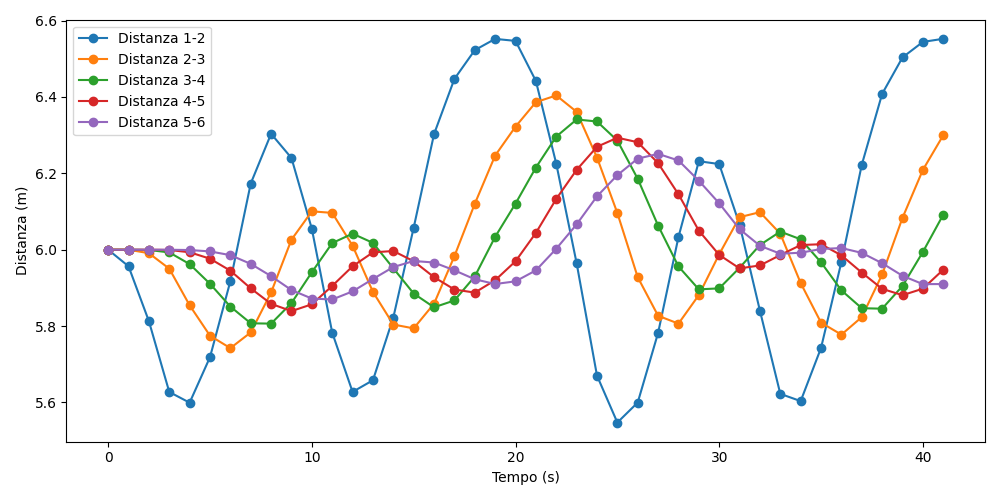
\includegraphics[width=0.96\textwidth]{images/5-experiment/velocity/distance_20-0-20-0-20.png}
    \caption{Distanze con velocità variabile tra $20\hspace{0.2em}m/s$ e $0\hspace{0.2em}m/s$.}
    \label{fig:20-0-variabvelocity-distance}
\end{figure}

\begin{figure}[H]
    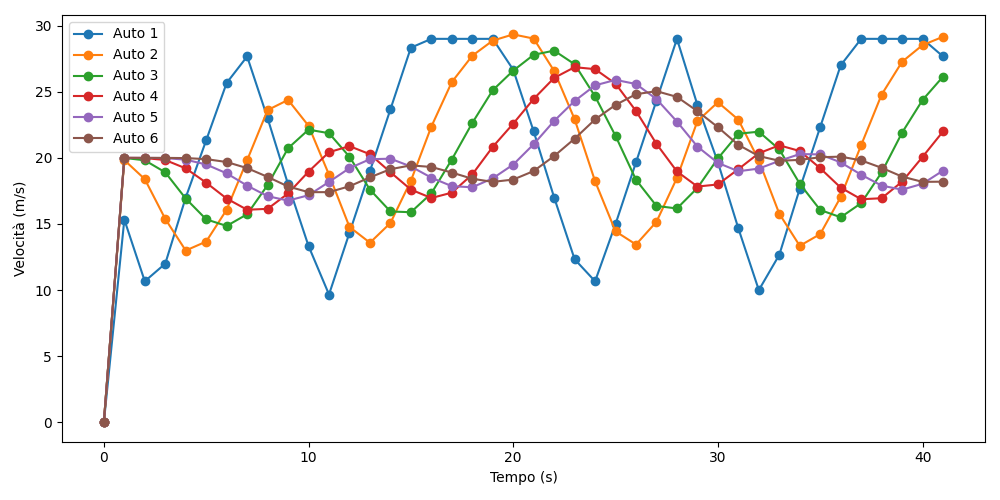
\includegraphics[width=0.96\textwidth]{images/5-experiment/velocity/velocity_20-0-20-0-20.png}
    \caption{Velocità con velocità variabile tra $20\hspace{0.2em}m/s$ e $0\hspace{0.2em}m/s$.}
    \label{fig:20-0-variabvelocity-velocity}
\end{figure}

\newpage

\begin{table}[h]
    \centering
    \begin{tabular}{|c|c|c|c|c|}
        \hline
        Velocità $t1$ & Velocità $t2$ & Velocità $t3$ &Velocità $t4$ &Velocità $t5$\\
        \hline
            $35\hspace{0.2em}m/s$ & $35\hspace{0.2em}m/s$ & $0\hspace{0.2em}m/s$ & $35\hspace{0.2em}m/s$ & $35\hspace{0.2em}m/s$ \\
        \hline
    \end{tabular}
\end{table}
\begin{table}[h]
    \centering
    \begin{tabular}{|c|c|c|c|}
        \hline
        N° auto & Distanza Iniziale & Distanza Target & Ritardo \\
        \hline
        $6$ & $6.0 m$ & $5.0 m$ & $0.2 s$ \\
        \hline
        $Time\hspace{0.2em}Headway$ & $\tau$ & $K_p$ & $K_d$  \\
        \hline
        $0.5$ & $0.1$ & $0.2$ & $0.7$ \\
        \hline
    \end{tabular}
\end{table}

\begin{figure}[H]
    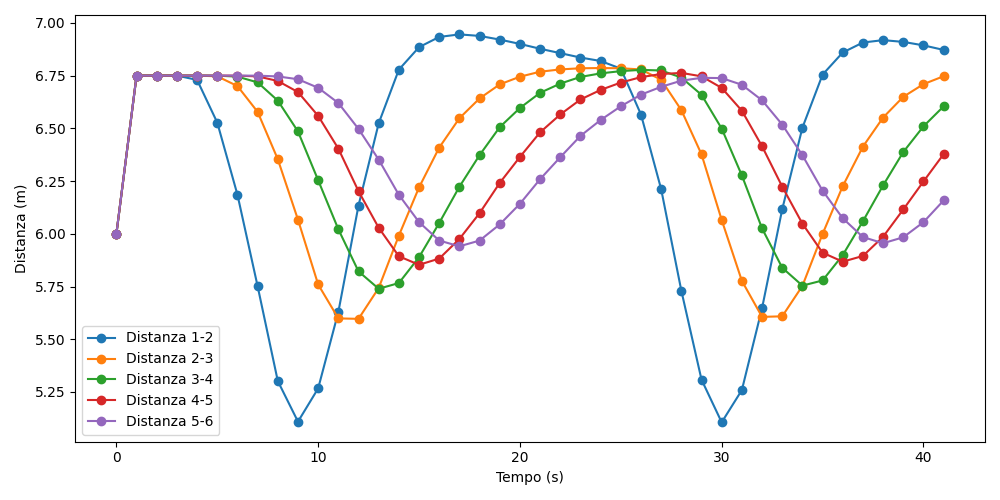
\includegraphics[width=0.96\textwidth]{images/5-experiment/velocity/distance_35-35-0-35-35.png}
    \caption{Distanze con velocità variabile tra $35\hspace{0.2em}m/s$ e $0\hspace{0.2em}m/s$.}
    \label{fig:35-35-0-variabvelocity-distance}
\end{figure}

\begin{figure}[H]
    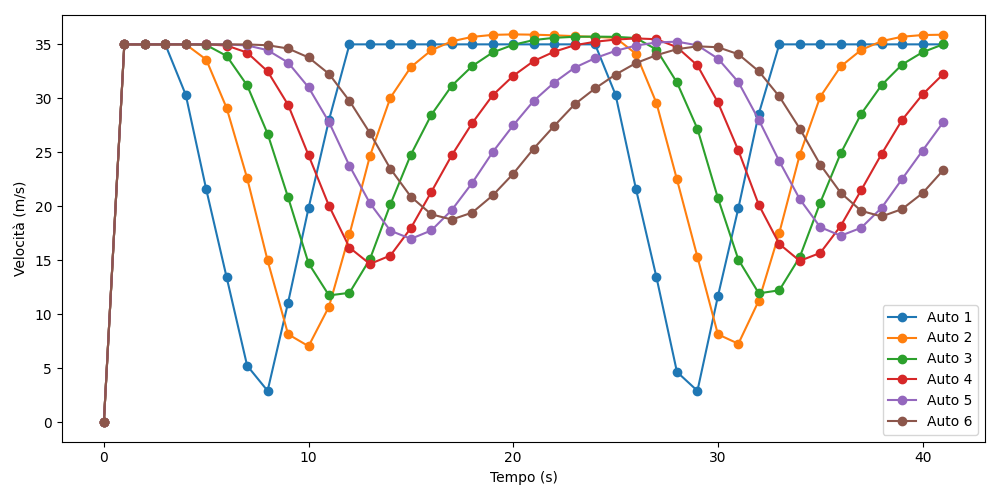
\includegraphics[width=0.96\textwidth]{images/5-experiment/velocity/velocity_35-35-0-35-35.png}
    \caption{Velocità con velocità variabile tra $35\hspace{0.2em}m/s$ e $0\hspace{0.2em}m/s$.}
    \label{fig:35-35-0-variabvelocity-velocity}
\end{figure}

\newpage


% VELOCITÀ NON PARAMETRI DEFAULT%

\subsubsection{Velocità con parametri diversi da quelli di default}

\begin{table}[h]
    \centering
    \begin{tabular}{|c|c|c|c|c|}
        \hline
        Velocità $t1$ & Velocità $t2$ & Velocità $t3$ &Velocità $t4$ &Velocità $t5$\\
        \hline
            $15\hspace{0.2em}m/s$ & $15\hspace{0.2em}m/s$ & $15\hspace{0.2em}m/s$ & $15\hspace{0.2em}m/s$ & $15\hspace{0.2em}m/s$ \\
        \hline
    \end{tabular}
\end{table}
\begin{table}[h]
    \centering
    \begin{tabular}{|c|c|c|c|}
        \hline
        N° auto & Distanza Iniziale & Distanza Target & Ritardo \\
        \hline
        $10$ & $6.0 m$ & $5.0 m$ & $0.2 s$ \\
        \hline
        $Time\hspace{0.2em}Headway$ & $\tau$ & $K_p$ & $K_d$  \\
        \hline
        $0.1$ & $0.1$ & $0.2$ & $0.7$ \\
        \hline
    \end{tabular}
\end{table}

\begin{figure}[H]
    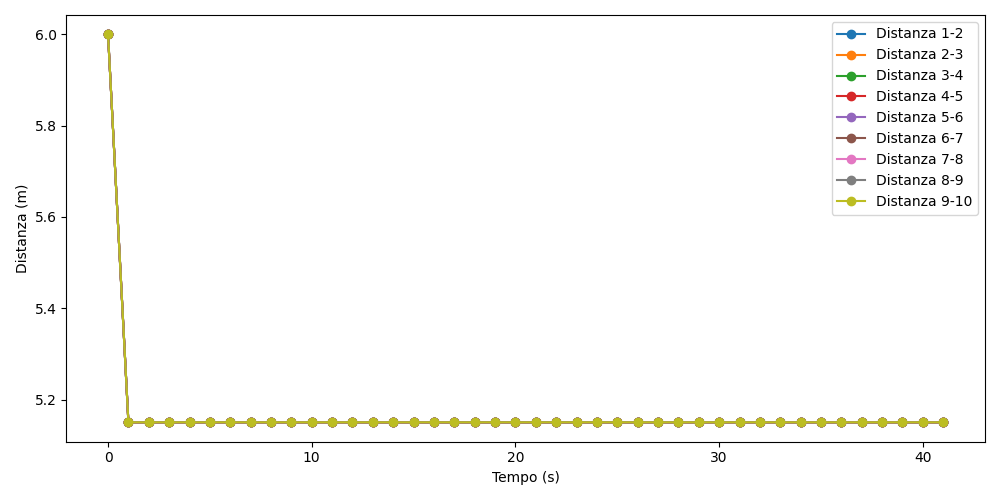
\includegraphics[width=0.96\textwidth]{images/5-experiment/compost/distance_a.png}
    \caption{Distanze con velocità costante a $15\hspace{0.2em}m/s$.}
    \label{fig:a-compost-distance}
\end{figure}

\begin{figure}[H]
    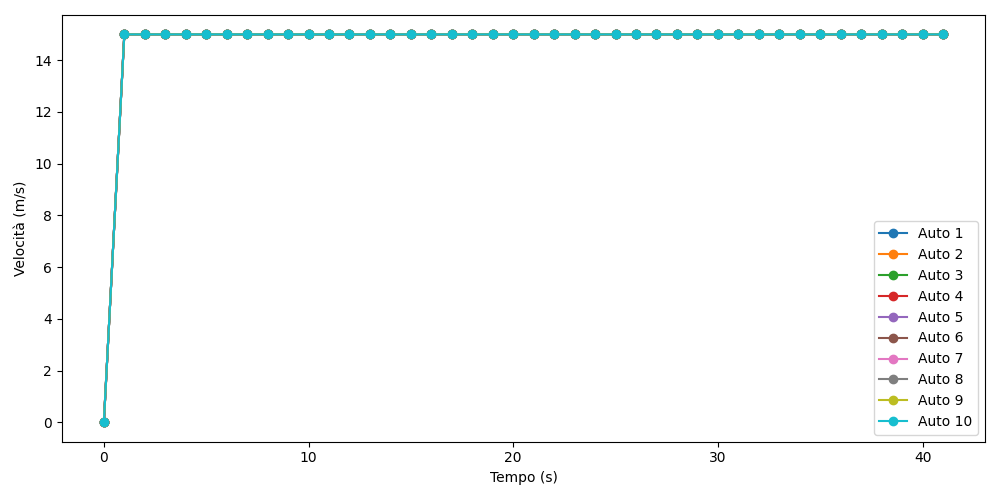
\includegraphics[width=0.96\textwidth]{images/5-experiment/compost/velocity_a.png}
    \caption{Velocità con velocità costante a $15\hspace{0.2em}m/s$.}
    \label{fig:a-compost-velocity}
\end{figure}

\vspace*{\fill}
\newpage
\vspace*{\fill}
\begin{table}[h]
    \centering
    \begin{tabular}{|c|c|c|c|c|}
        \hline
        Velocità $t1$ & Velocità $t2$ & Velocità $t3$ &Velocità $t4$ &Velocità $t5$\\
        \hline
            $25\hspace{0.2em}m/s$ & $25\hspace{0.2em}m/s$ & $25\hspace{0.2em}m/s$ & $25\hspace{0.2em}m/s$ & $25\hspace{0.2em}m/s$ \\
        \hline
    \end{tabular}
\end{table}
\begin{table}[h]
    \centering
    \begin{tabular}{|c|c|c|c|}
        \hline
        N° auto & Distanza Iniziale & Distanza Target & Ritardo \\
        \hline
        $10$ & $3.0 m$ & $2.0 m$ & $0.2 s$ \\
        \hline
        $Time\hspace{0.2em}Headway$ & $\tau$ & $K_p$ & $K_d$  \\
        \hline
        $0.1$ & $0.1$ & $0.2$ & $0.7$ \\
        \hline
    \end{tabular}
\end{table}

\begin{figure}[H]
    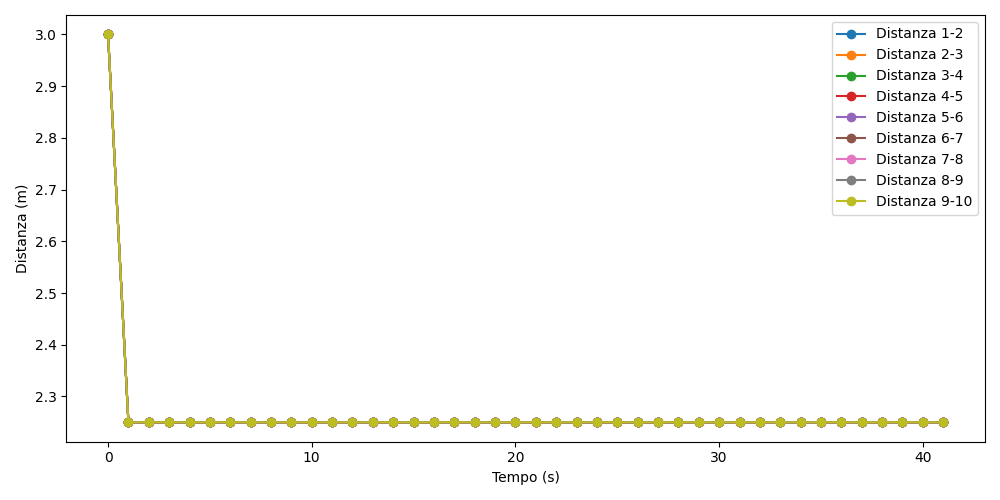
\includegraphics[width=0.96\textwidth]{images/5-experiment/compost/distance_b.png}
    \caption{Distanze con velocità costante a $25\hspace{0.2em}m/s$.}
    \label{fig:b-compost-distance}
\end{figure}

\begin{figure}[H]
    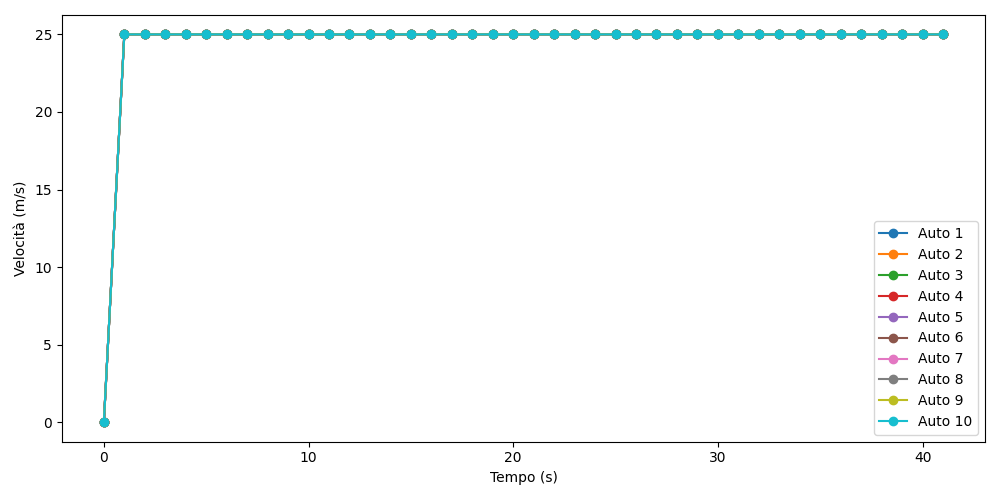
\includegraphics[width=0.96\textwidth]{images/5-experiment/compost/velocity_b.png}
    \caption{Velocità con velocità costante a $25\hspace{0.2em}m/s$.}
    \label{fig:b-compost-velocity}
\end{figure}
\vspace*{\fill}
\newpage

\begin{table}[h]
    \centering
    \begin{tabular}{|c|c|c|c|c|}
        \hline
        Velocità $t1$ & Velocità $t2$ & Velocità $t3$ &Velocità $t4$ &Velocità $t5$\\
        \hline
            $25\hspace{0.2em}m/s$ & $25\hspace{0.2em}m/s$ & $15\hspace{0.2em}m/s$ & $25\hspace{0.2em}m/s$ & $25\hspace{0.2em}m/s$ \\
        \hline
    \end{tabular}
\end{table}

\begin{table}[h]
    \centering
    \begin{tabular}{|c|c|c|c|}
        \hline
        N° auto & Distanza Iniziale & Distanza Target & Ritardo \\
        \hline
        $10$ & $3.0 m$ & $5.0 m$ & $0.2 s$ \\
        \hline
        $Time\hspace{0.2em}Headway$ & $\tau$ & $K_p$ & $K_d$  \\
        \hline
        $0.1$ & $0.1$ & $0.2$ & $0.7$ \\
        \hline
    \end{tabular}
\end{table}

\begin{figure}[H]
    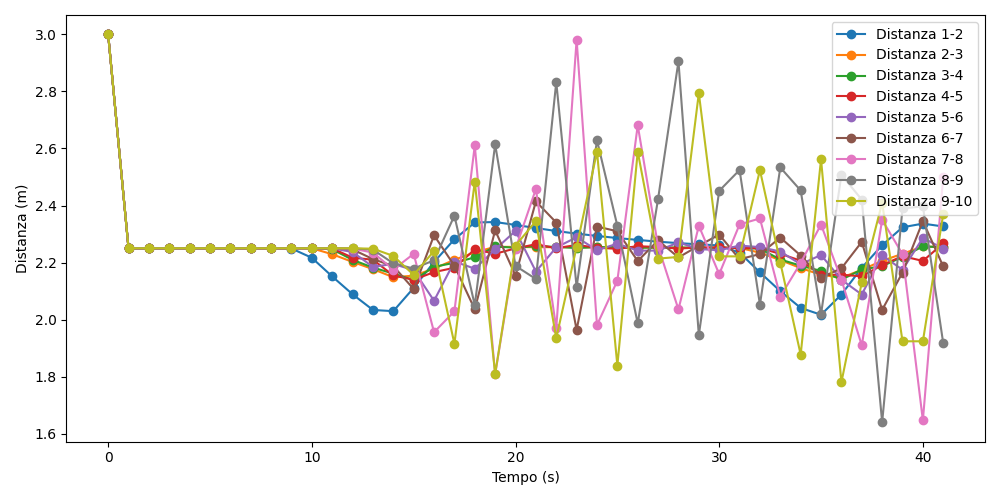
\includegraphics[width=0.96\textwidth]{images/5-experiment/compost/distance_c.png}
    \caption{Distanze con velocità variabile tra $15\hspace{0.2em}m/s$ e $25\hspace{0.2em}m/s$.}
    \label{fig:c-compost-distance}
\end{figure}

\begin{figure}[H]
    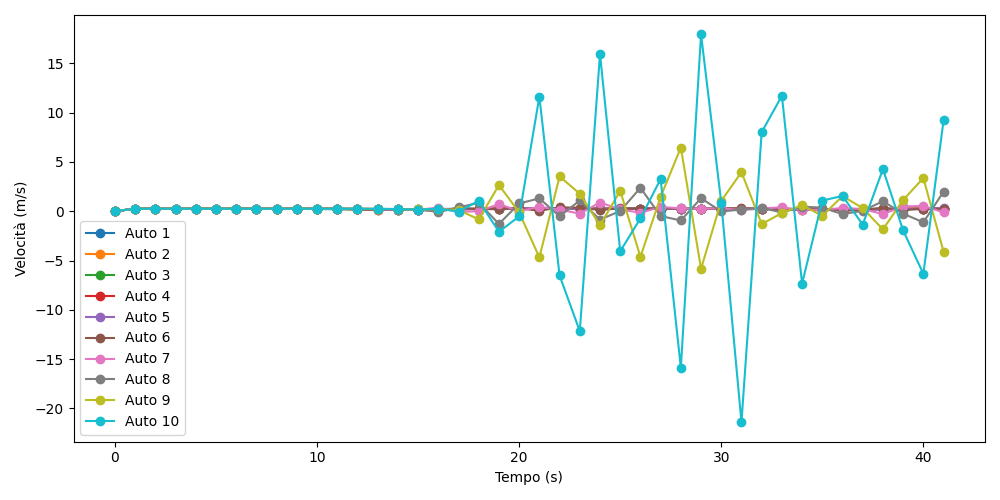
\includegraphics[width=0.96\textwidth]{images/5-experiment/compost/velocity_c.png}
    \caption{Velocità con velocità variabile tra $15\hspace{0.2em}m/s$ e $25\hspace{0.2em}m/s$.}
    \label{fig:c-compost-velocity}
\end{figure}

\newpage


% MODELLO INSTABILE %

\subsection{Modello instabile}

% DELAY %

\subsubsection{Ritardo di comunicazione}
\vspace*{\fill}
\begin{table}[h]
    \centering
    \begin{tabular}{|c|c|c|c|}
        \hline
        N° auto & Distanza Iniziale & Distanza Target & Ritardo \\
        \hline
        $6$ & $6.0 m$ & $5.0 m$ & $1.5 s$ \\
        \hline
        $Time\hspace{0.2em}Headway$ & $\tau$ & $K_p$ & $K_d$  \\
        \hline
        $0.5$ & $0.1$ & $0.2$ & $0.7$ \\
        \hline
    \end{tabular}
\end{table}

\begin{figure}[H]
    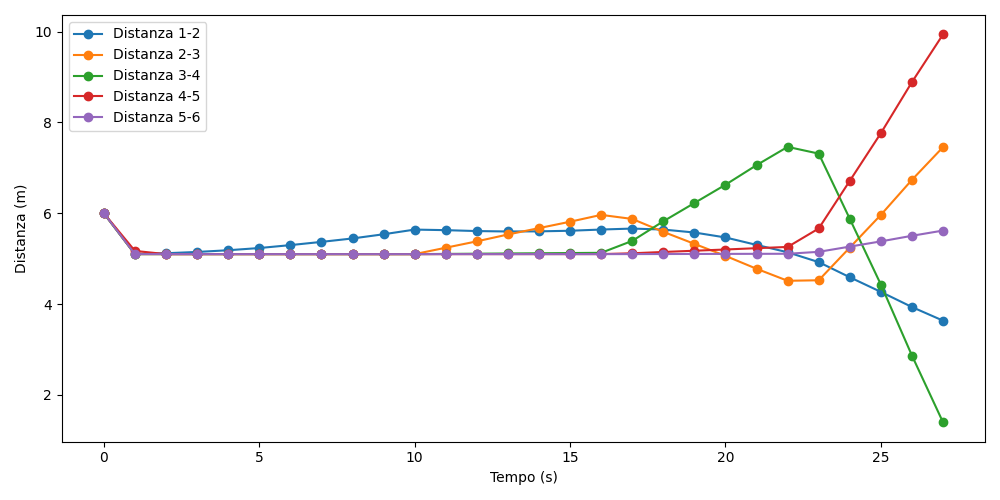
\includegraphics[width=0.96\textwidth]{images/5-experiment/delay/distance_1,5+.png}
    \caption{Distanze con ritardo a $1.5 s$.}
    \label{fig:1.5-delay-distance}
\end{figure}

\begin{figure}[H]
    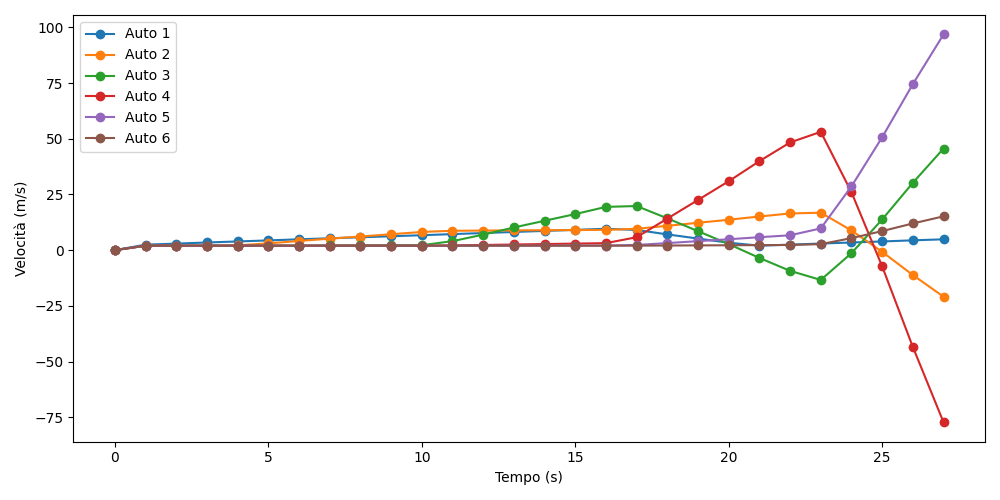
\includegraphics[width=0.96\textwidth]{images/5-experiment/delay/velocity_1,5+.png}
    \caption{Velocità con ritardo a $1.5 s$.}
    \label{fig:1.5-delay-velocity}
\end{figure}
\vspace*{\fill}
\newpage
\vspace*{\fill}
\begin{table}[h]
    \centering
    \begin{tabular}{|c|c|c|c|}
        \hline
        N° auto & Distanza Iniziale & Distanza Target & Ritardo \\
        \hline
        $6$ & $6.0 m$ & $5.0 m$ & $2 s$ \\
        \hline
        $Time\hspace{0.2em}Headway$ & $\tau$ & $K_p$ & $K_d$  \\
        \hline
        $0.5$ & $0.1$ & $0.2$ & $0.7$ \\
        \hline
    \end{tabular}
\end{table}

\begin{figure}[H]
    \includegraphics[width=0.96\textwidth]{images/5-experiment/delay/distance_2+.png}
    \caption{Distanze con ritardo a $2 s$.}
    \label{fig:2-delay-distance}
\end{figure}

\begin{figure}[H]
    \includegraphics[width=0.96\textwidth]{images/5-experiment/delay/velocity_2+.png}
    \caption{Velocità con ritardo a $2 s$.}
    \label{fig:2-delay-velocity}
\end{figure}
\vspace*{\fill}
\newpage

% VELOCITÀ PARAMETRI NON DEFAULT%

\subsubsection{Velocità con parametri diversi da quelli di default}

\begin{table}[h]
    \centering
    \begin{tabular}{|c|c|c|c|c|}
        \hline
        Velocità $t1$ & Velocità $t2$ & Velocità $t3$ &Velocità $t4$ &Velocità $t5$\\
        \hline
            $35\hspace{0.2em}m/s$ & $20\hspace{0.2em}m/s$ & $0\hspace{0.2em}m/s$ & $15\hspace{0.2em}m/s$ & $35\hspace{0.2em}m/s$ \\
        \hline
    \end{tabular}
\end{table}

\begin{table}[h]
    \centering
    \begin{tabular}{|c|c|c|c|}
        \hline
        N° auto & Distanza Iniziale & Distanza Target & Ritardo \\
        \hline
        $6$ & $3.0 m$ & $2.0 m$ & $0.2 s$ \\
        \hline
        $Time\hspace{0.2em}Headway$ & $\tau$ & $K_p$ & $K_d$  \\
        \hline
        $0.05$ & $0.1$ & $0.2$ & $0.7$ \\
        \hline
    \end{tabular}
\end{table}

\begin{figure}[H]
    \includegraphics[width=0.96\textwidth]{images/5-experiment/compost/distance_d+.png}
    \caption{Distanze con velocità variabile tra $0\hspace{0.2em}m/s$ e $35\hspace{0.2em}m/s$.}
    \label{fig:d-compost-distance}
\end{figure}

\begin{figure}[H]
    \includegraphics[width=0.96\textwidth]{images/5-experiment/compost/velocity_d+.png}
    \caption{Velocità con velocità variabile tra $0\hspace{0.2em}m/s$ e $35\hspace{0.2em}m/s$.}
    \label{fig:d-compost-velocity}
\end{figure}

\newpage

\begin{table}[h]
    \centering
    \begin{tabular}{|c|c|c|c|c|}
        \hline
        Velocità $t1$ & Velocità $t2$ & Velocità $t3$ &Velocità $t4$ &Velocità $t5$\\
        \hline
                $35\hspace{0.2em}m/s$ & $20\hspace{0.2em}m/s$ & $0\hspace{0.2em}m/s$ & $15\hspace{0.2em}m/s$ & $35\hspace{0.2em}m/s$ \\
        \hline
    \end{tabular}
\end{table}

\begin{table}[h]
    \centering
    \begin{tabular}{|c|c|c|c|}
        \hline
        N° auto & Distanza Iniziale & Distanza Target & Ritardo \\
        \hline
        $7$ & $4.5 m$ & $3.5 m$ & $1.0 s$ \\
        \hline
        $Time\hspace{0.2em}Headway$ & $\tau$ & $K_p$ & $K_d$  \\
        \hline
        $0.3$ & $0.1$ & $0.2$ & $0.7$ \\
        \hline
    \end{tabular}
\end{table}

\begin{figure}[H]
    \includegraphics[width=0.96\textwidth]{images/5-experiment/compost/distance_e+.png}
    \caption{Distanze con velocità variabile tra $0\hspace{0.2em}m/s$ e $35\hspace{0.2em}m/s$.}
    \label{fig:e-compost-distance}
\end{figure}

\begin{figure}[H]
    \includegraphics[width=0.96\textwidth]{images/5-experiment/compost/velocity_e+.png}
    \caption{Velocità con velocità variabile tra $0\hspace{0.2em}m/s$ e $35\hspace{0.2em}m/s$.}
    \label{fig:e-compost-velocity}
\end{figure}




% ESEMPIO 2 IMMAGINI
% \begin{figure}[H]
%     \begin{minipage}[t]{0.5\textwidth}
%         \centering
%         \includegraphics[width=\linewidth]{images/5-experiment/car-number/distance_10.png}
%         \caption{Image 1}
%         \label{fig:sub1}
%     \end{minipage}
%     \hfill
%     \begin{minipage}[t]{0.5\textwidth}
%         \centering
%         \includegraphics[width=\linewidth]{images/5-experiment/car-number/velocity_10.png}
%         \caption{Image 2}
%         \label{fig:sub2}
%     \end{minipage}
%     \label{fig:two_images}
% \end{figure}